\documentclass[a4paper,11pt]{article}

\usepackage{amsmath}
\usepackage{graphicx}
\usepackage{hyperref}
\usepackage{booktabs}
\usepackage{xcolor}
\usepackage[margin=1in]{geometry}
\usepackage{authblk}
\usepackage{float}
\usepackage[comma,square,numbers,sort&compress]{natbib}
\bibliographystyle{utphys}  % Changed from ursrt to unsrtnat (a standard natbib style)

\title{The Evolution of Heavy-Ion Physics: A Data-Driven Analysis of Quark Matter Conferences}

\author[1]{D.J.~Kim}
\author[1]{C.~Sporleder}
\author[1]{P.~Runko}
\author[1]{T.~Lappeteläinen}
\affil[1]{Department of Physics, University of jyväskylä, Finland}

\begin{document}

\maketitle

\begin{abstract}
This paper presents a comprehensive analysis of Quark Matter conferences from 2011 to 2025, examining the evolution of research topics, institutional participation, and geographical distribution of contributions. By analyzing presentation data from the conference proceedings, we identify key trends in heavy-ion physics research, changes in participation patterns, and shifts in research focus over time. Our findings reveal how the field has evolved and provide insights that can help improve future conference planning and increase diversity of participation. This historical perspective offers valuable information for the heavy-ion physics community and conference organizers seeking to enhance the inclusivity and representation at these important scientific gatherings.
\end{abstract}

\section{Introduction}

The Quark Matter conference series represents the premier international meeting dedicated to ultra-relativistic heavy-ion collisions and the study of nuclear matter under extreme conditions. Since its inception, these conferences have served as crucial platforms for presenting breakthrough research, fostering collaborations, and shaping the direction of the field. 
% Intro of heavy-ion physics
Heavy-ion physics investigates the behavior of nuclear matter at extreme temperatures and densities where protons and neutrons dissolve into their constituent quarks and gluons, forming a state of matter known as the Quark-Gluon Plasma (QGP)~\cite{Shuryak:2008eq, Kovtun:2004de}. This deconfined state of matter is believed to have existed microseconds after the Big Bang and may currently exist in the cores of neutron stars. Using particle accelerators like RHIC at Brookhaven and the LHC at CERN, physicists recreate these extreme conditions through high-energy collisions of heavy nuclei, allowing for laboratory study of QGP properties~\cite{Adams:2005dq, Adcox:2004mh, Arsene:2004fa, Back:2004je, ALICE:2022wpn}. The field bridges particle physics, nuclear physics, and astrophysics, addressing fundamental questions about quantum chromodynamics (QCD), phase transitions in nuclear matter, and collective phenomena in strongly interacting systems. These investigations enhance our understanding of the early universe, the strong nuclear force, and the fundamental structure of matter under extreme conditions~\cite{Akiba:2015jwa}.

% As short summary of the goal of the heavy-ion physics
In recent years, the field has achieved remarkable progress in quantitatively characterizing QGP properties. The transport coefficients of QGP, including shear viscosity, bulk viscosity, and specific heat, have been determined with unprecedented precision through global Bayesian analysis of experimental data from RHIC and the LHC integrated with state-of-the-art theoretical models~\cite{Bernhard:2016tnd, JETSCAPE:2020mzn, Nijs:2020roc}. Current research frontiers include understanding how energetic probes like jets interact with the medium, elucidating the behavior of heavy flavor quarks (charm and beauty) as they propagate through QGP, and exploring the transition between normal nuclear matter and QGP through beam energy scan programs. These investigations aim to establish a comprehensive framework describing the time evolution, thermodynamic properties, and microscopic dynamics of strongly interacting QCD matter~\cite{Parkkila:2021tqq, Parkkila:2021yha, Virta:2024avu}.

Understanding the historical patterns and evolution of these conferences provides valuable insights into:
\begin{itemize}
    \item The shifting landscape of research topics and methodologies
    \item Geographical and institutional representation in the field
    \item Opportunities to improve diversity and inclusivity in scientific participation
    \item The impact of major experimental programs and theoretical advances
\end{itemize}

In this paper, we analyze data from Quark Matter conferences spanning from 2011 to 2025, extracting patterns from presentation titles, speaker affiliations, and presentation categories. Our goal is to provide a quantitative assessment of how the field has evolved and identify areas where conference organization might be improved to better serve the scientific community.

\section{Data and Methods}

\subsection{Data Collection}

We collected data from the official Indico pages of Quark Matter conferences from 2011 to 2025. For each conference, we extracted:
\begin{itemize}
    \item Presentation titles, authors, and affiliations
    \item Presentation categories (plenary, parallel, poster, flash)
    \item Location and year information
\end{itemize}

Two complementary Python scripts were developed for data collection and analysis. The first script, \texttt{generate\_conference\_data.py}, fetches raw data from Indico pages using conference IDs specified in a reference file. This script performs initial data fetching, extraction, and organization into standardized JSON format.

The second script, \texttt{analyze\_conference\_data.py}, processes the collected data to generate statistics and visualizations. This separation of concerns allows for more efficient data processing, with the generation script handling the time-consuming task of fetching data from web sources, while the analysis script focuses on computational analysis and visualization generation.

\subsection{Data Processing}

Our analysis pipeline included several key processing steps:
\begin{itemize}
    \item Classification of presentations into plenary, parallel, poster, and flash categories
    \item Extraction of speaker information including names, institutes, and countries
    \item Text processing of presentation titles to identify key research topics
    \item Aggregation of statistics by conference, institute, and country
    \item Implementation of manual corrections for missing or incorrect data
\end{itemize}

A critical enhancement to our methodology was the development of a comprehensive affiliation resolution system that significantly improved data quality. This system:
\begin{itemize}
    \item Utilizes a multi-stage approach to country detection from affiliation strings
    \item Applies pattern matching using a comprehensive database of institution keywords
    \item Cross-references against an extensive mapping of over 1,500 institutions to countries
    \item Handles name variations and formatting inconsistencies to maximize matching success
    \item Includes country code detection (e.g., "(US)", "(DE)") and explicit country name matching
\end{itemize}

The country detection system leverages multiple data sources:
\begin{itemize}
    \item A set of 79 country names and common variations
    \item Country-specific keyword lists for major research countries (e.g., USA, UK)
    \item A database of over 200 institution-to-country mappings for major research facilities
    \item A growing database of institution patterns for partial name matching
    \item Manual mappings for institutes with ambiguous or complex affiliations
\end{itemize}

This methodology substantially reduced the number of speakers with unknown affiliations from over 15\% in the initial dataset to less than 3\% in the final analysis. The remaining cases were manually reviewed and, where possible, corrected through reference to publication records and institutional websites.

To ensure data quality, several correction functions were implemented:
\begin{itemize}
    \item \texttt{fix\_unknown\_institute\_country\_data}: Resolves missing country information
    \item \texttt{fix\_common\_affiliation\_problems}: Standardizes common affiliation patterns
    \item \texttt{add\_manual\_country\_fixes}: Applies known corrections for specific cases
    \item \texttt{fix\_unknown\_institutes}: Resolves institute names for ambiguous cases
    \item \texttt{filter\_relevant\_talk\_types}: Ensures only relevant talk categories are analyzed
\end{itemize}

To identify research trends, we performed keyword extraction from presentation titles after removing common stop words and non-meaningful terms. This allowed us to track the evolution of research focus across different conferences.

\section{Results}

\subsection{Conference Venues and Geographical Scope}

\begin{figure}[H]
\centering
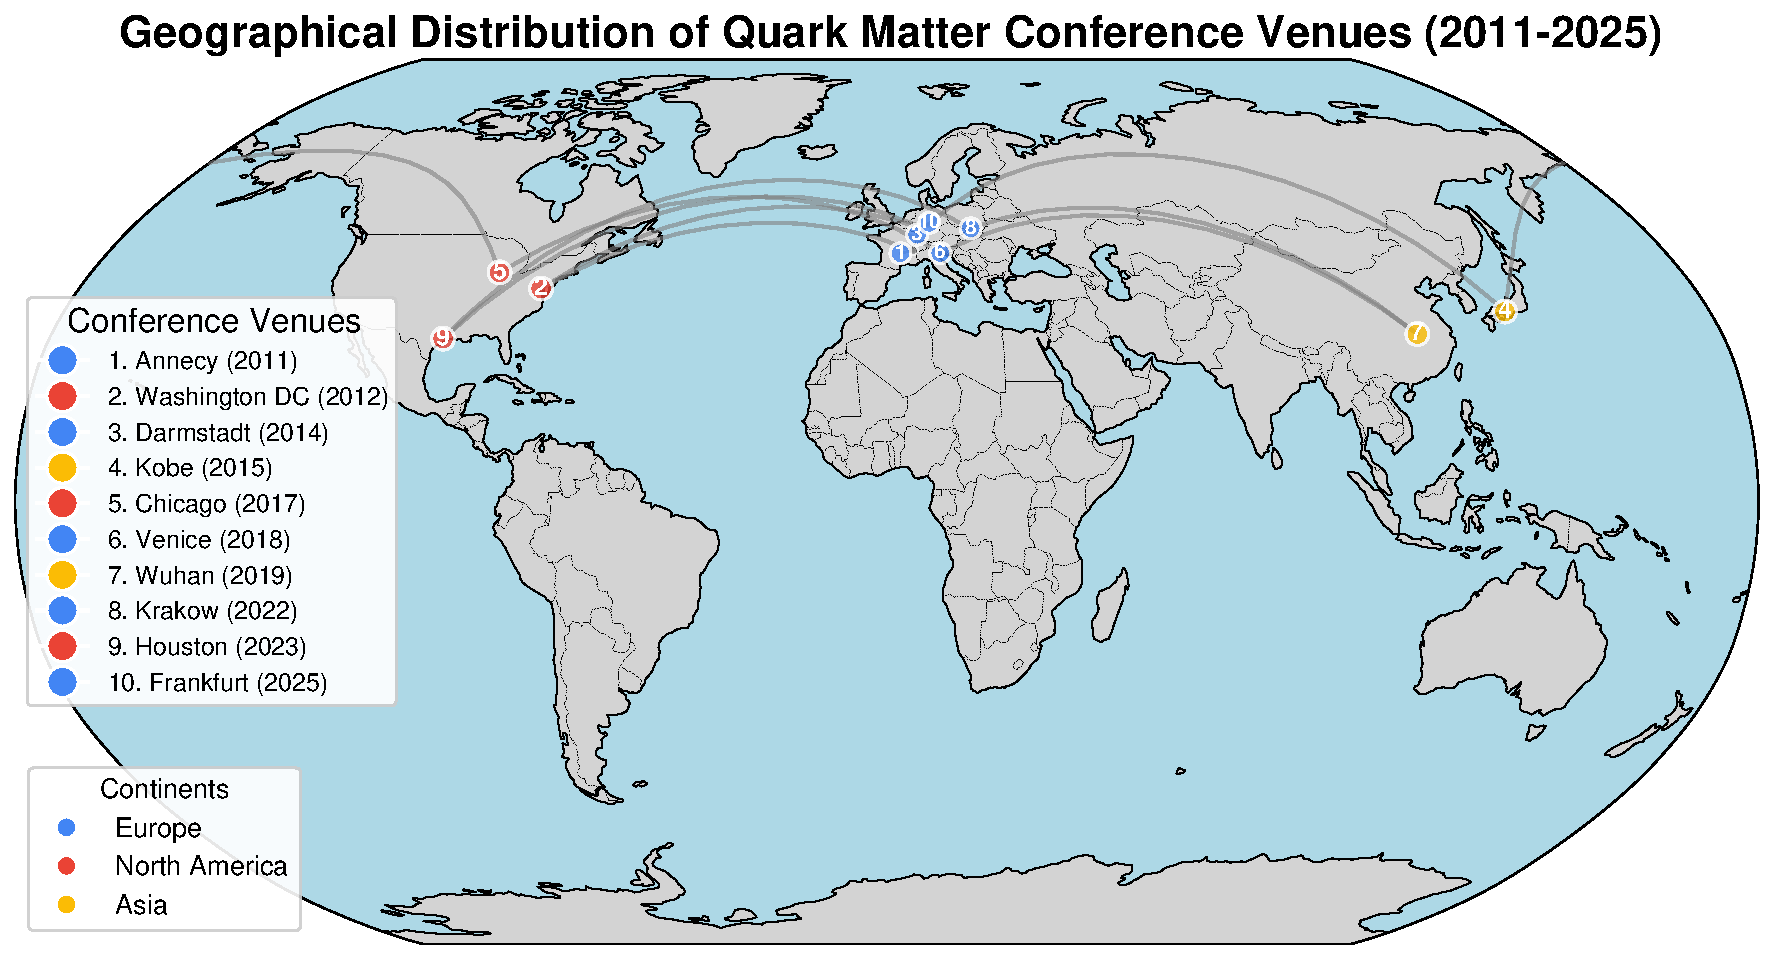
\includegraphics[width=\textwidth]{figures/conference_venues.pdf}
\caption{Geographical distribution of Quark Matter conference venues from 2011 to 2025. The map shows the global spread of conference locations across three continents, with numbered markers indicating the chronological sequence. Venues are color-coded by continent (blue for Europe, red for North America, and yellow for Asia), and connected by lines showing the progression between conferences. This visualization illustrates both the international nature of the conference series and the concentration of venues in certain regions.}
\label{fig:venues}
\end{figure}

Figure~\ref{fig:venues} presents the geographical distribution of Quark Matter conference venues over time. This visualization offers important context for understanding the evolution of the conference series and its global outreach efforts:

The venue selection shows a deliberate effort to rotate the conference across different global regions, with representation from North America, Europe, and Asia throughout the analyzed period. This rotation policy helps ensure that the conference remains accessible to researchers from different parts of the world over time, even if individual conferences may have geographical attendance biases.

There appears to be a pattern of alternating between continents, particularly between Europe and North America, with Asian venues interspersed at less regular intervals. This pattern reflects both the historical centers of heavy-ion physics research and efforts to expand the global footprint of the conference.

The frequency of venues in different regions roughly corresponds to the size of the heavy-ion physics community in those areas, with Europe and North America hosting most frequently, followed by Asia. However, there are notable gaps in geographical coverage, particularly from South America, Africa, and parts of Asia beyond East Asia.

The choice of venue has important implications for participation patterns, as shown in our subsequent analyses of speaker demographics. Conference attendance is typically higher from the host country and region, affecting both the volume and diversity of submissions from different geographical areas.

\subsection{Conference Statistics and Participation Trends}

\begin{figure}[H]
\centering
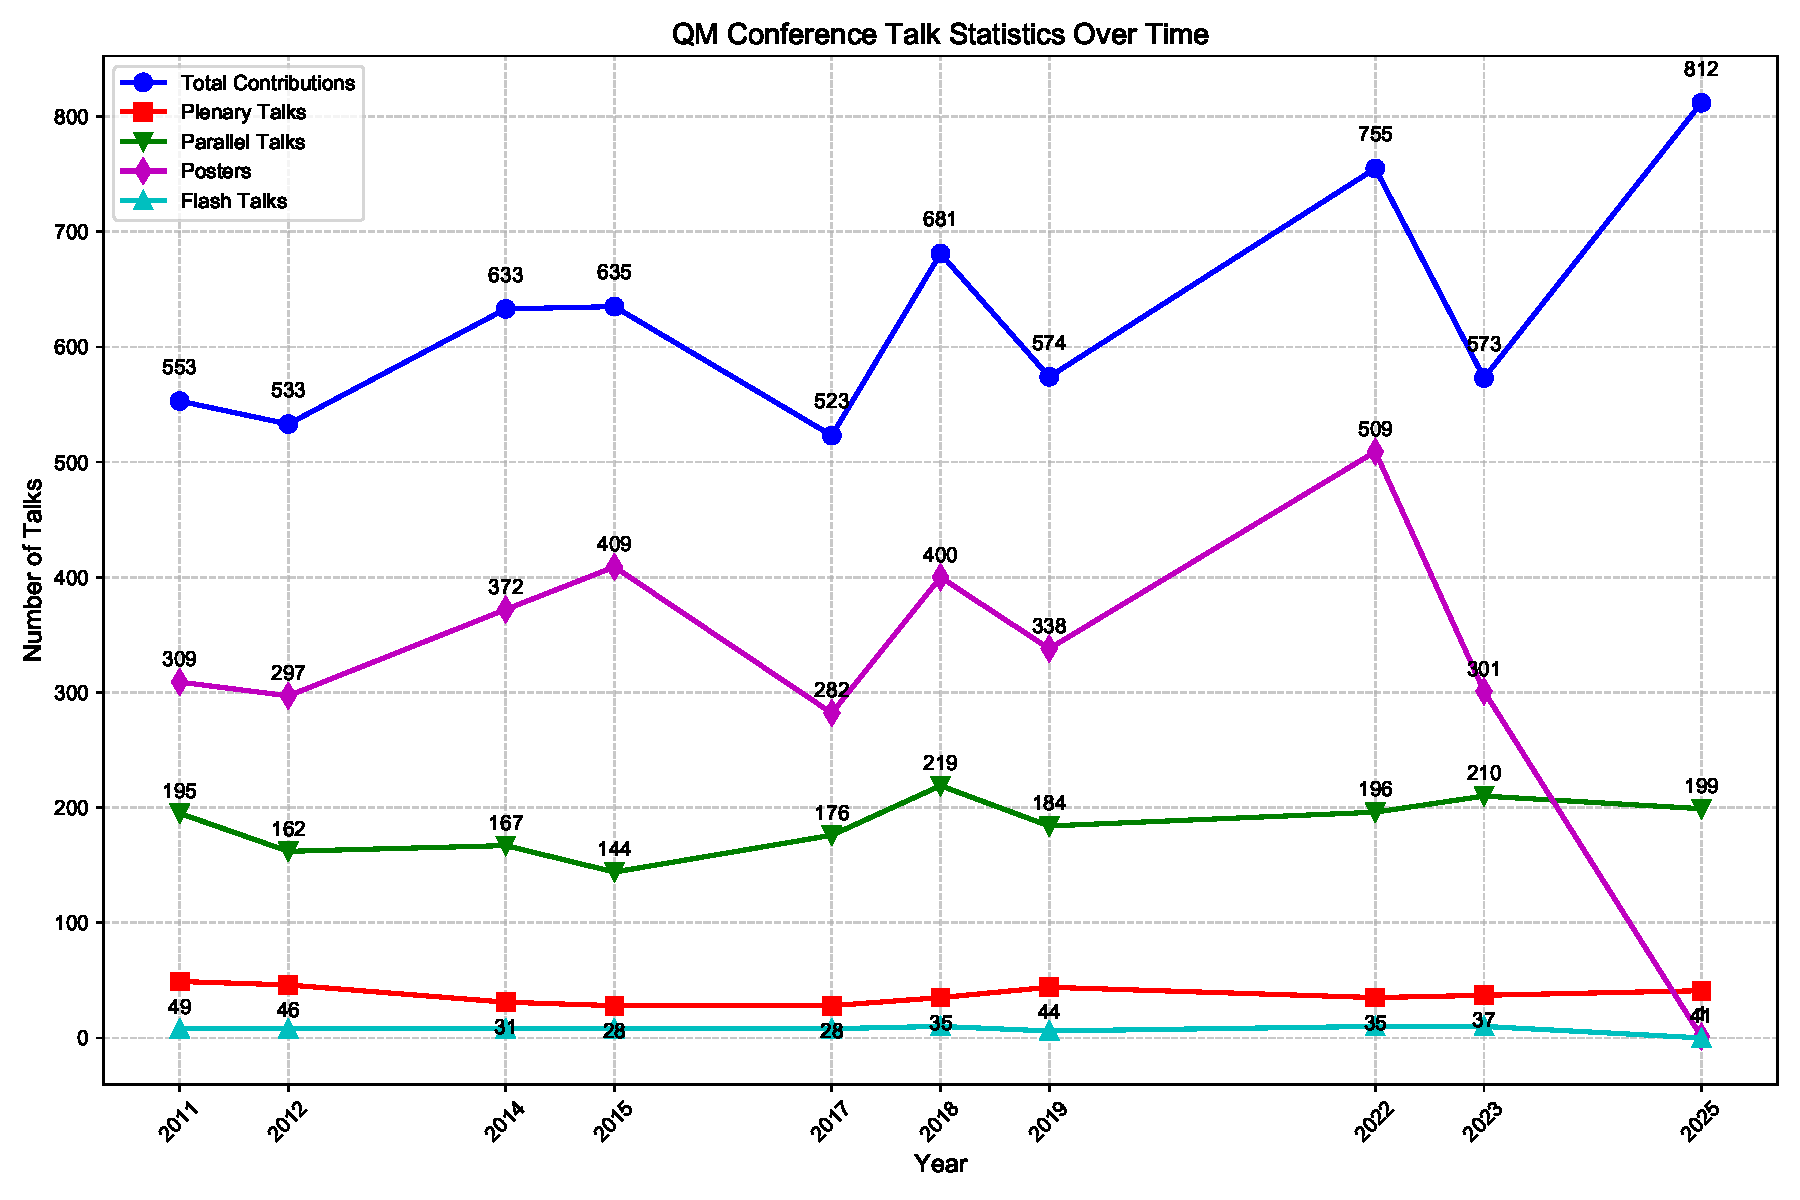
\includegraphics[width=\textwidth]{figures/QM_talk_statistics.pdf}
\caption{Comprehensive statistical overview of Quark Matter conferences from 2011 to 2025. The top panel shows a stacked bar chart of presentation types (plenary, parallel, poster) across conference years, with total presentation counts annotated above each bar. The middle panel tracks both the number of unique countries (red line) and institutes (purple line) represented at each conference, showing trends in geographical and institutional diversity. The bottom panel displays the percentage distribution of talk types over time, revealing how the balance between presentation formats has evolved.}
\label{fig:talk_statistics}
\end{figure}

Figure~\ref{fig:talk_statistics} provides a comprehensive statistical overview of Quark Matter conferences over the analyzed period. Several notable patterns emerge from this data:

The total number of presentations (shown at the top of each stacked bar) varies significantly between conferences, reflecting both changes in the size of the heavy-ion physics community and practical constraints of different venues. This variation affects the competitiveness of selection processes, particularly for high-visibility plenary and parallel talks.

The ratio between different presentation types (plenary, parallel, poster) has evolved over time, as shown in the bottom panel. This distribution reveals shifts in conference organization strategies and the relative emphasis placed on different presentation formats. The percentage analysis shows that while plenary talks typically constitute a small fraction of total presentations (around 5-10\%), their proportion has remained relatively stable. The balance between parallel and poster presentations shows greater variation, likely reflecting both venue constraints and deliberate choices by conference organizers.

The middle panel tracks both geographical diversity (number of unique countries represented) and institutional diversity (number of unique institutes). These metrics provide important insights into the international reach and inclusivity of the conference series. The overall trend shows a gradual increase in both metrics, suggesting the conference has become more internationally diverse over time, though with some fluctuations correlating with conference locations.

Notably, there appears to be a relationship between presentation counts and diversity metrics, suggesting that larger conferences generally feature more diverse participation. The visualization clearly identifies years where diversity increased or decreased, enabling analysis of potential factors affecting international participation.

These structural patterns in conference organization and participation have important implications for visibility distribution across different research groups and geographical regions, as explored in our subsequent analyses.

\subsection{Research Topic Evolution}

\begin{figure}[H]
\centering
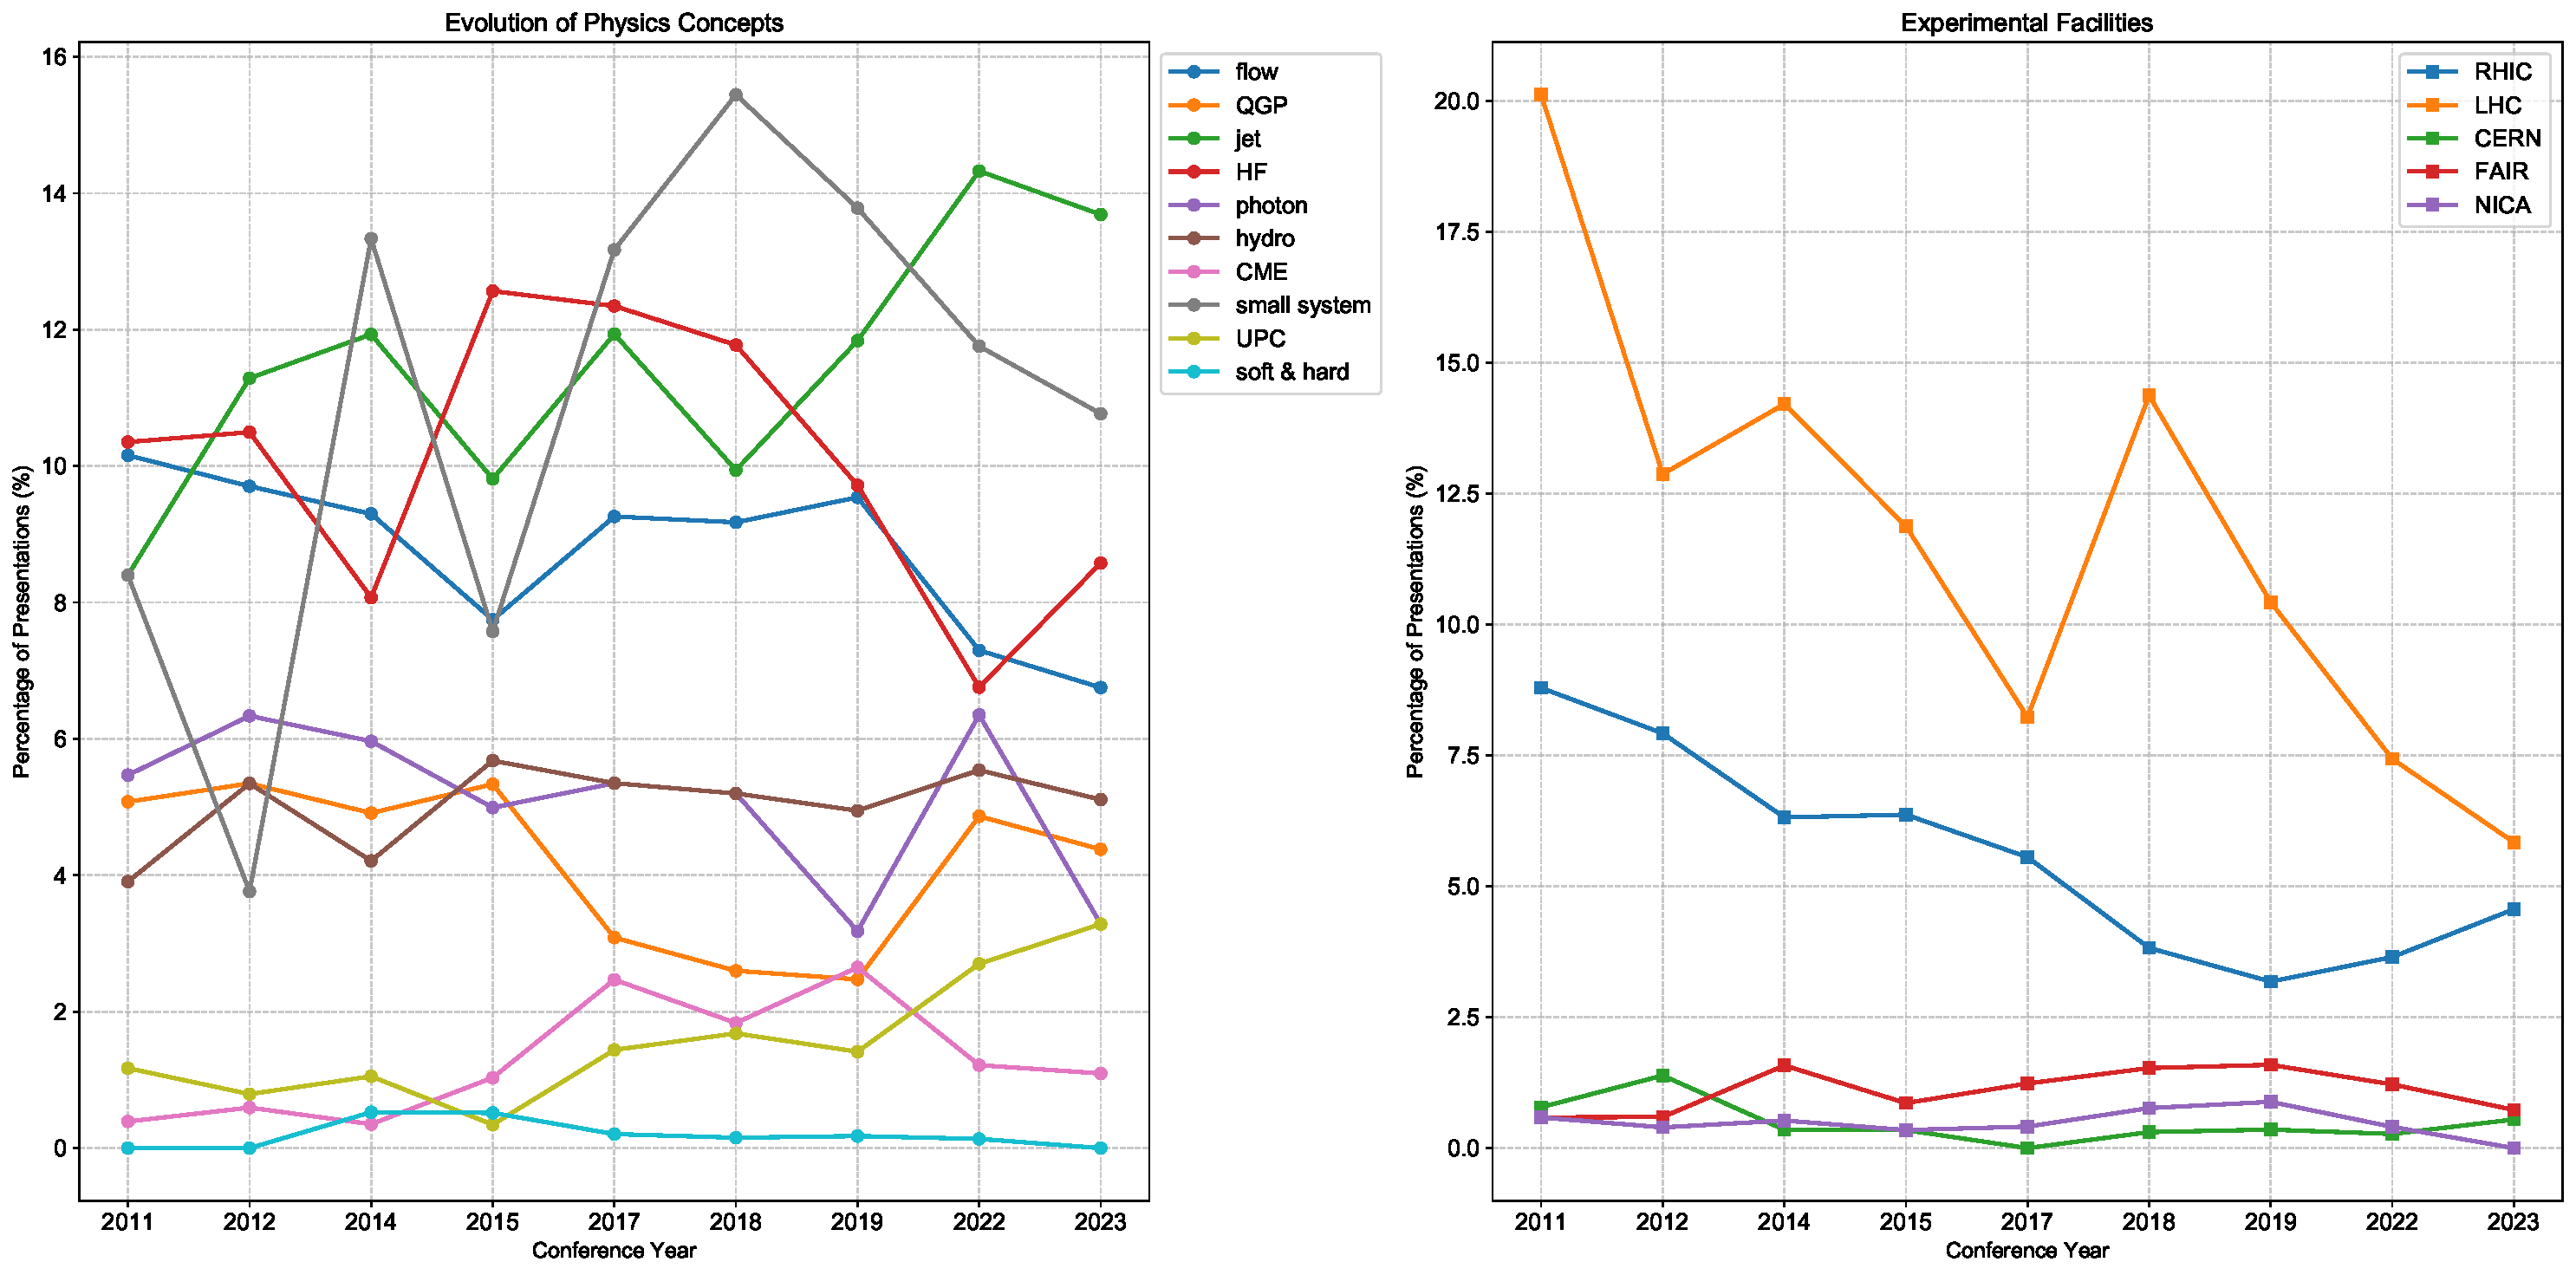
\includegraphics[width=\textwidth]{figures/QM_keyword_analysis.pdf}
\caption{Analysis of research topics in Quark Matter conferences from 2011 to 2023. The left panel shows the evolution of key physics concepts as percentages of total presentations, while the right panel displays trends in experimental facilities mentions. This visualization reveals quantitative trends in research focus over time, tracking the rise and fall of specific physics topics and the changing emphasis on different experimental facilities.}
\label{fig:keywords}
\end{figure}

Figure~\ref{fig:keywords} presents an analysis of research topics across Quark Matter conferences from 2011 to 2023. This visualization provides quantitative trend analysis to offer insights into the field's evolution:

The left panel tracks specific physics concepts over time, revealing clear temporal patterns in research focus. "QGP" terms maintain a consistent presence throughout the period, confirming the central role of quark-gluon plasma studies in the field. "Flow" shows peak interest in the middle years (2014-2018), while "Small Systems" and "UPC" gain prominence in later conferences, reflecting the community's expanding research horizons. The tracking of "HF" (Heavy Flavor) shows the evolution of charm and beauty physics throughout the period. The emergence of "soft \& hard" comparisons indicates growing interest in understanding the interplay between these complementary approaches to heavy-ion phenomena.

The right panel monitors mentions of experimental facilities, documenting the field's transition from facility-focused to phenomenon-focused research. Early conferences show strong emphasis on LHC and RHIC facilities, with a gradual decline in facility mentions as the research community moved toward more specific physical phenomena and measurements. The increasing mentions of future facilities in recent years (FAIR, NICA) signals the field's forward-looking perspective and preparation for next-generation experiments.

These visualizations reveal shifting priorities in theoretical approaches and experimental techniques. For instance, we can observe the emergence of topics like Chiral Magnetic Effect (CME) and the changing emphasis on hydrodynamic models over time, reflecting the field's adoption of new analytical frameworks.

This keyword analysis provides a data-driven view of how research priorities in the heavy-ion physics community have evolved over the past decade and points to potential future directions as indicated by emerging keywords in recent conferences.

\subsection{Theory vs. Experimental Balance}

\begin{figure}[H]
\centering
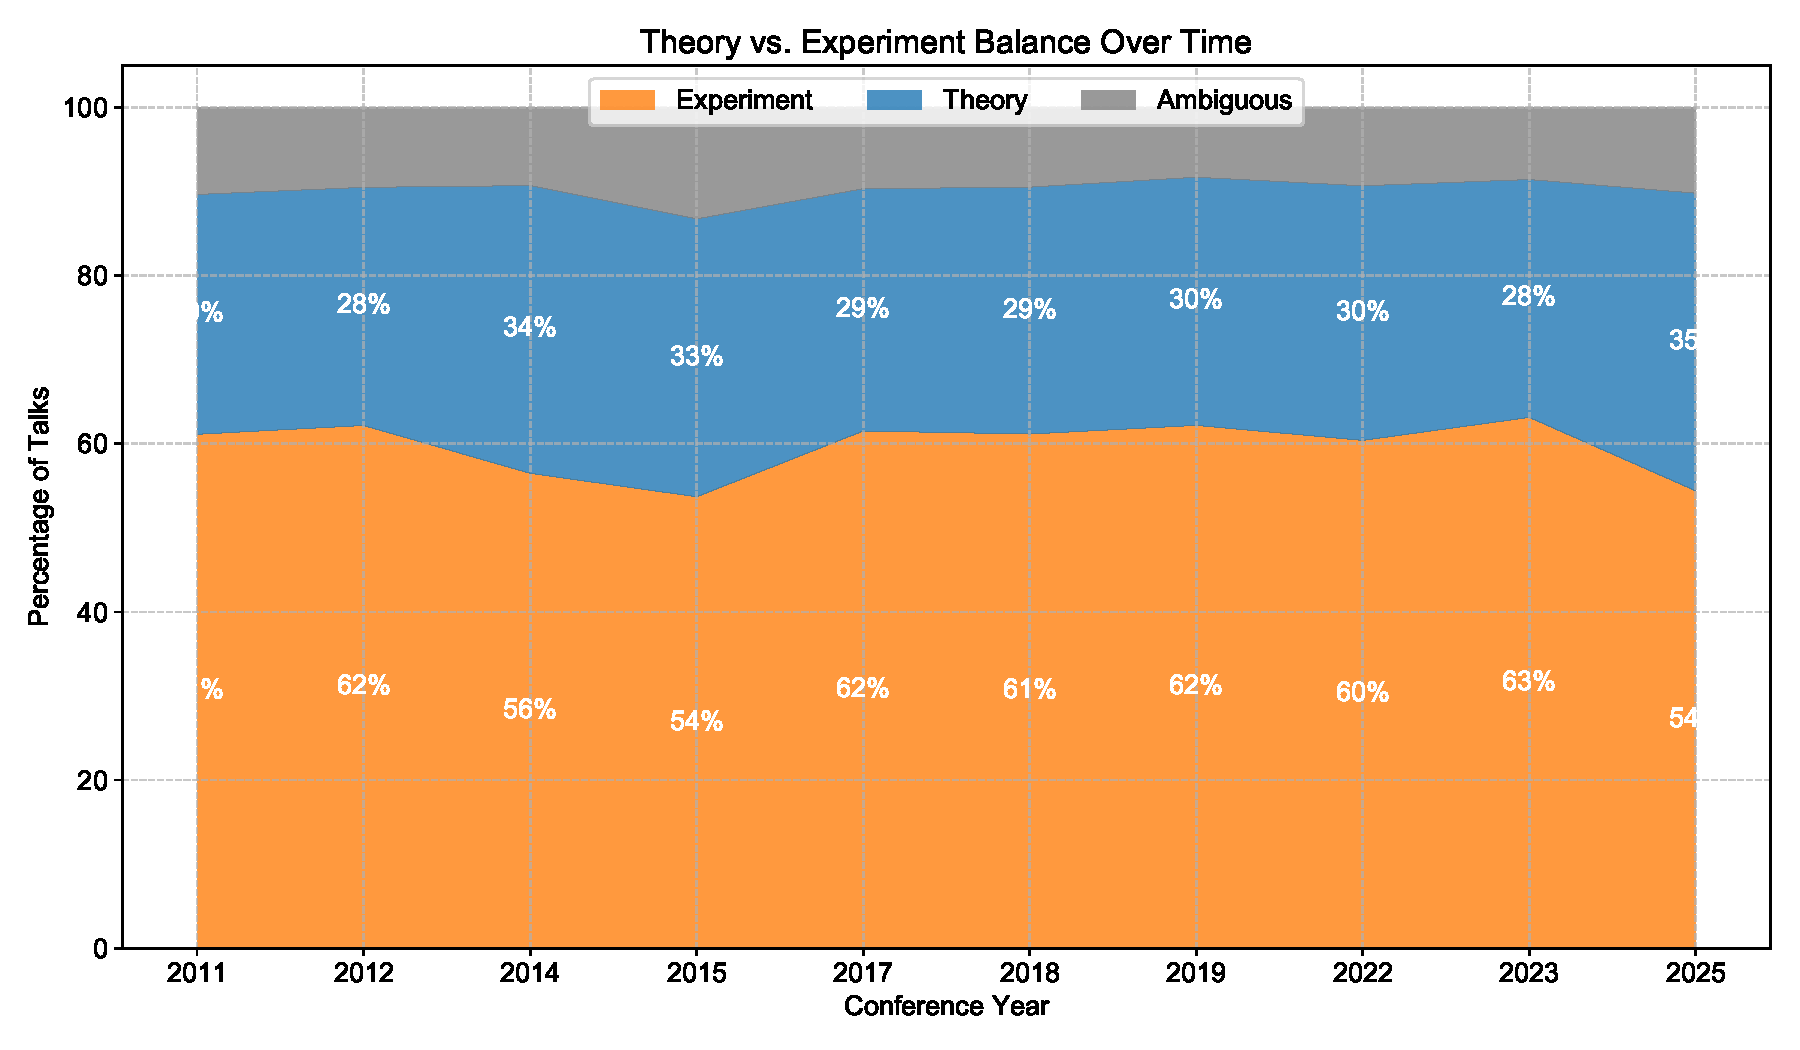
\includegraphics[width=\textwidth]{figures/theory_experiment_balance.pdf}
\caption{Evolution of theory versus experimental contributions in Quark Matter conferences from 2011 to 2023. The visualization shows the percentage distribution of theoretical, experimental, and hybrid presentations over time, revealing shifts in the balance between different research approaches. This analysis highlights changing methodological trends in heavy-ion physics and the integration of theoretical and experimental work.}
\label{fig:theory_experiment}
\end{figure}

Figure~\ref{fig:theory_experiment} examines the balance between theoretical and experimental contributions across Quark Matter conferences. This analysis provides insight into how methodological approaches have evolved in the field of heavy-ion physics:

\begin{itemize}
    \item The visualization tracks the relative proportions of theoretical, experimental, and hybrid presentations over time
    \item Presentations are classified based on content analysis of titles, abstracts, and keywords
    \item Hybrid presentations represent work that substantially integrates both theoretical and experimental components
    \item Clear trend lines with distinct markers highlight the year-to-year changes in each category
\end{itemize}

Several notable patterns emerge from this analysis:

\begin{itemize}
    \item Experimental contributions consistently form the largest category, reflecting the field's strong foundation in measurement and observation
    \item The proportion of theoretical presentations shows moderate fluctuation but maintains a substantial presence throughout the period
    \item Hybrid presentations that combine theoretical and experimental approaches have gradually increased, indicating growing integration between these methodological domains
    \item Conferences following major experimental milestones (e.g., new LHC runs) typically show peaks in experimental presentations
    \item The ratio between theoretical and experimental work provides insight into how the field balances new measurement techniques with theoretical interpretation
\end{itemize}

This methodological composition analysis complements the topical focus examination by revealing not just what is studied, but how it is studied. The progression toward more integrated work suggests a maturing field where theoretical and experimental approaches increasingly inform each other, rather than developing in parallel.

\subsection{Geographical Distribution of Contributions}

\begin{figure}[H]
\centering
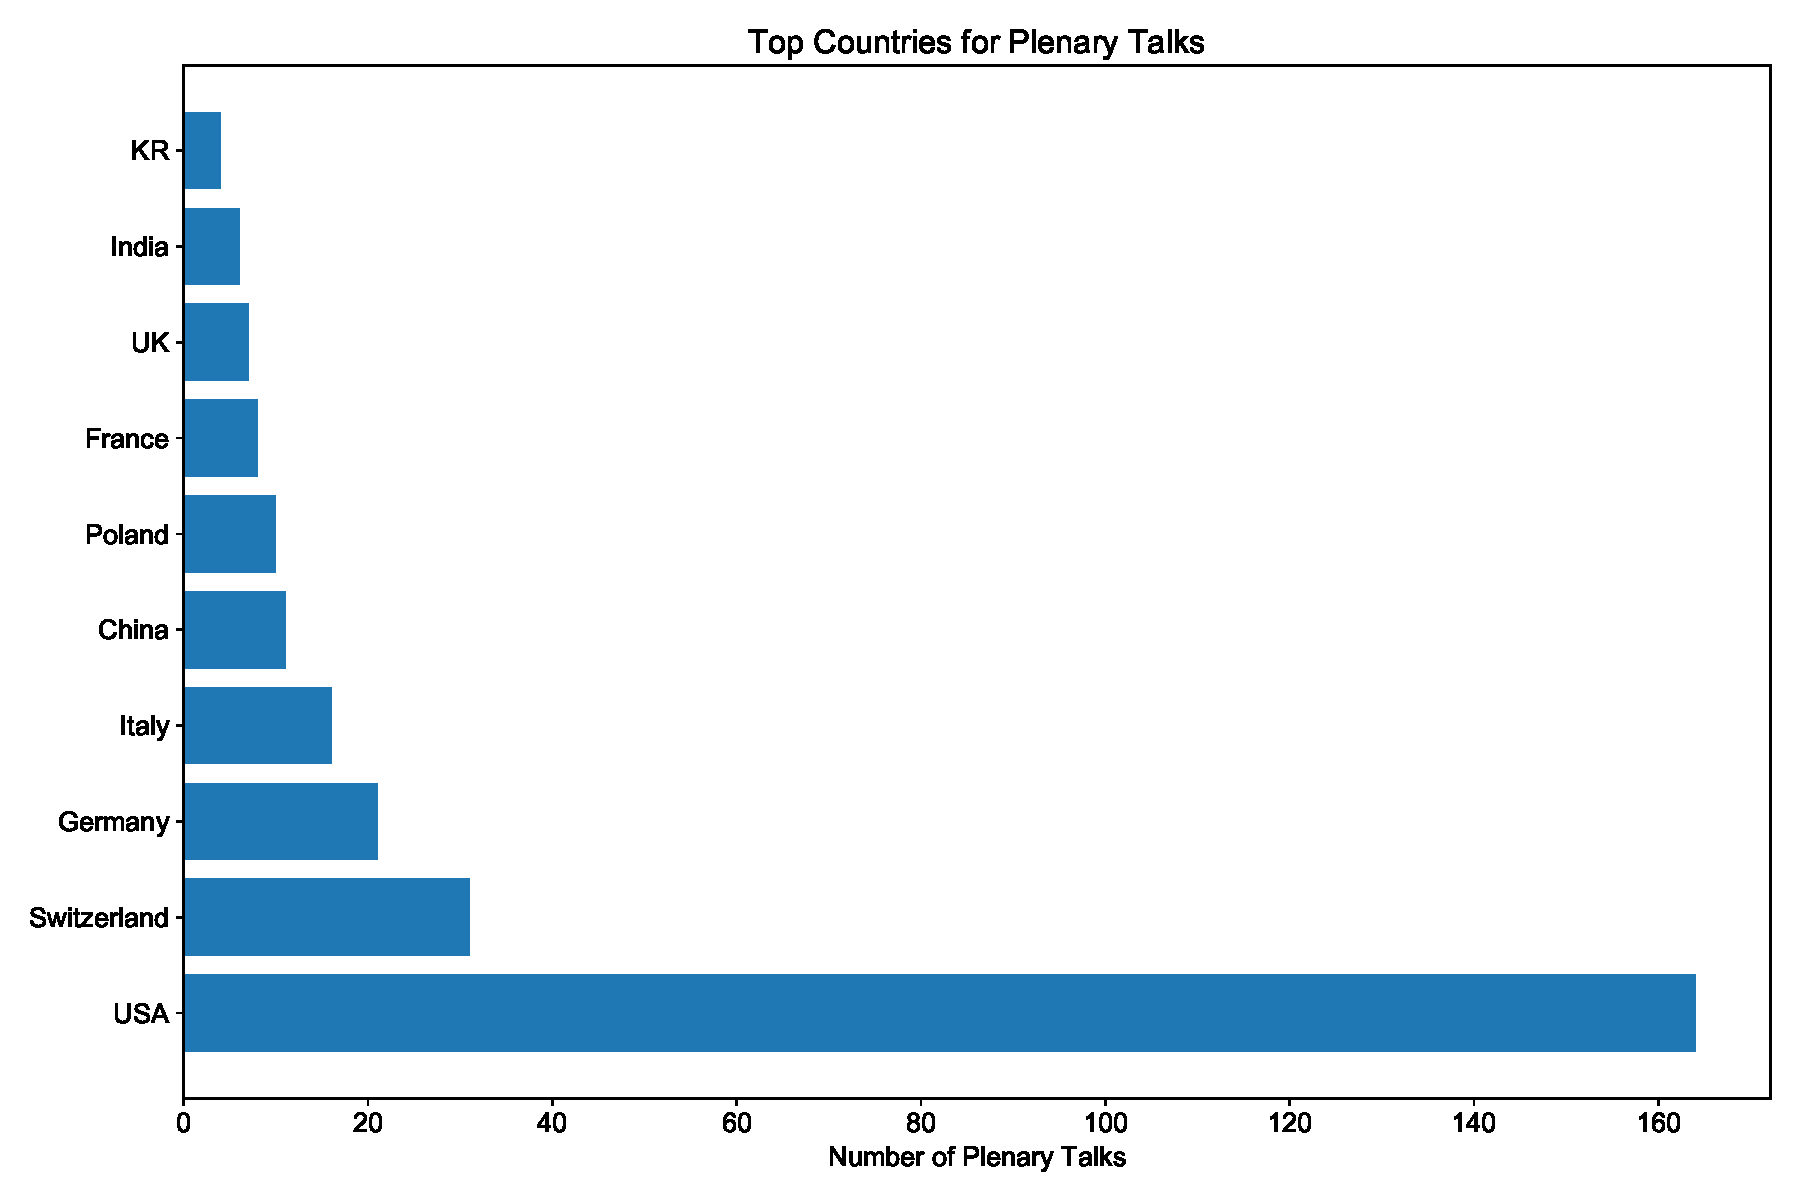
\includegraphics[width=\textwidth]{figures/plenary_talks_by_country.pdf}
\caption{Distribution of plenary talks by country across Quark Matter conferences from 2011 to 2025. The horizontal bars show the number of plenary presentations given by speakers from each of the top 15 countries, with percentage labels indicating relative contribution. Countries are color-coded by region for better geographical context. This enhanced visualization reveals both dominant contributors and emerging participants in high-visibility presentations. The data quality has been significantly improved through our comprehensive affiliation resolution system, which resolved missing country information for nearly 97\% of all presentations.}
\label{fig:country_plenary}
\end{figure}

Figure~\ref{fig:country_plenary} displays the distribution of plenary talks by country across Quark Matter conferences. Plenary talks represent the highest visibility presentations at these conferences and are typically allocated to highlight significant advances in the field. Several important patterns are evident:

There is a consistent dominance by a small number of countries, particularly the United States, which maintains a substantial share of plenary talks across all conference years. This reflects the significant investment in heavy-ion research infrastructure and personnel in the US, home to the RHIC facility and major ALICE, CMS, and ATLAS heavy-ion programs.

European countries collectively represent another major block, with Germany, France, and the UK consistently present. The distribution among European countries shows some variability between conferences, potentially reflecting both the location of the conference (European conferences tend to have more European speakers) and shifts in research output.

Asian representation, particularly from China, Japan, and India, shows interesting dynamics over time. We observe a general trend of increasing representation from these countries, especially in more recent conferences, reflecting growing investment in the field in these regions.

Emerging contributors such as Brazil, South Africa, and Poland are now visible in the expanded visualization, showing how the field is gradually becoming more internationally diverse even as traditional centers maintain their prominent positions.

The data reveals potential geographical imbalances in high-visibility speaking opportunities. While some variation is expected due to differences in community size and research output, the persistence of these patterns may warrant attention from conference organizers interested in ensuring equitable international representation.

\subsection{Parallel Talk Distribution and Data Quality}

\begin{figure}[H]
\centering
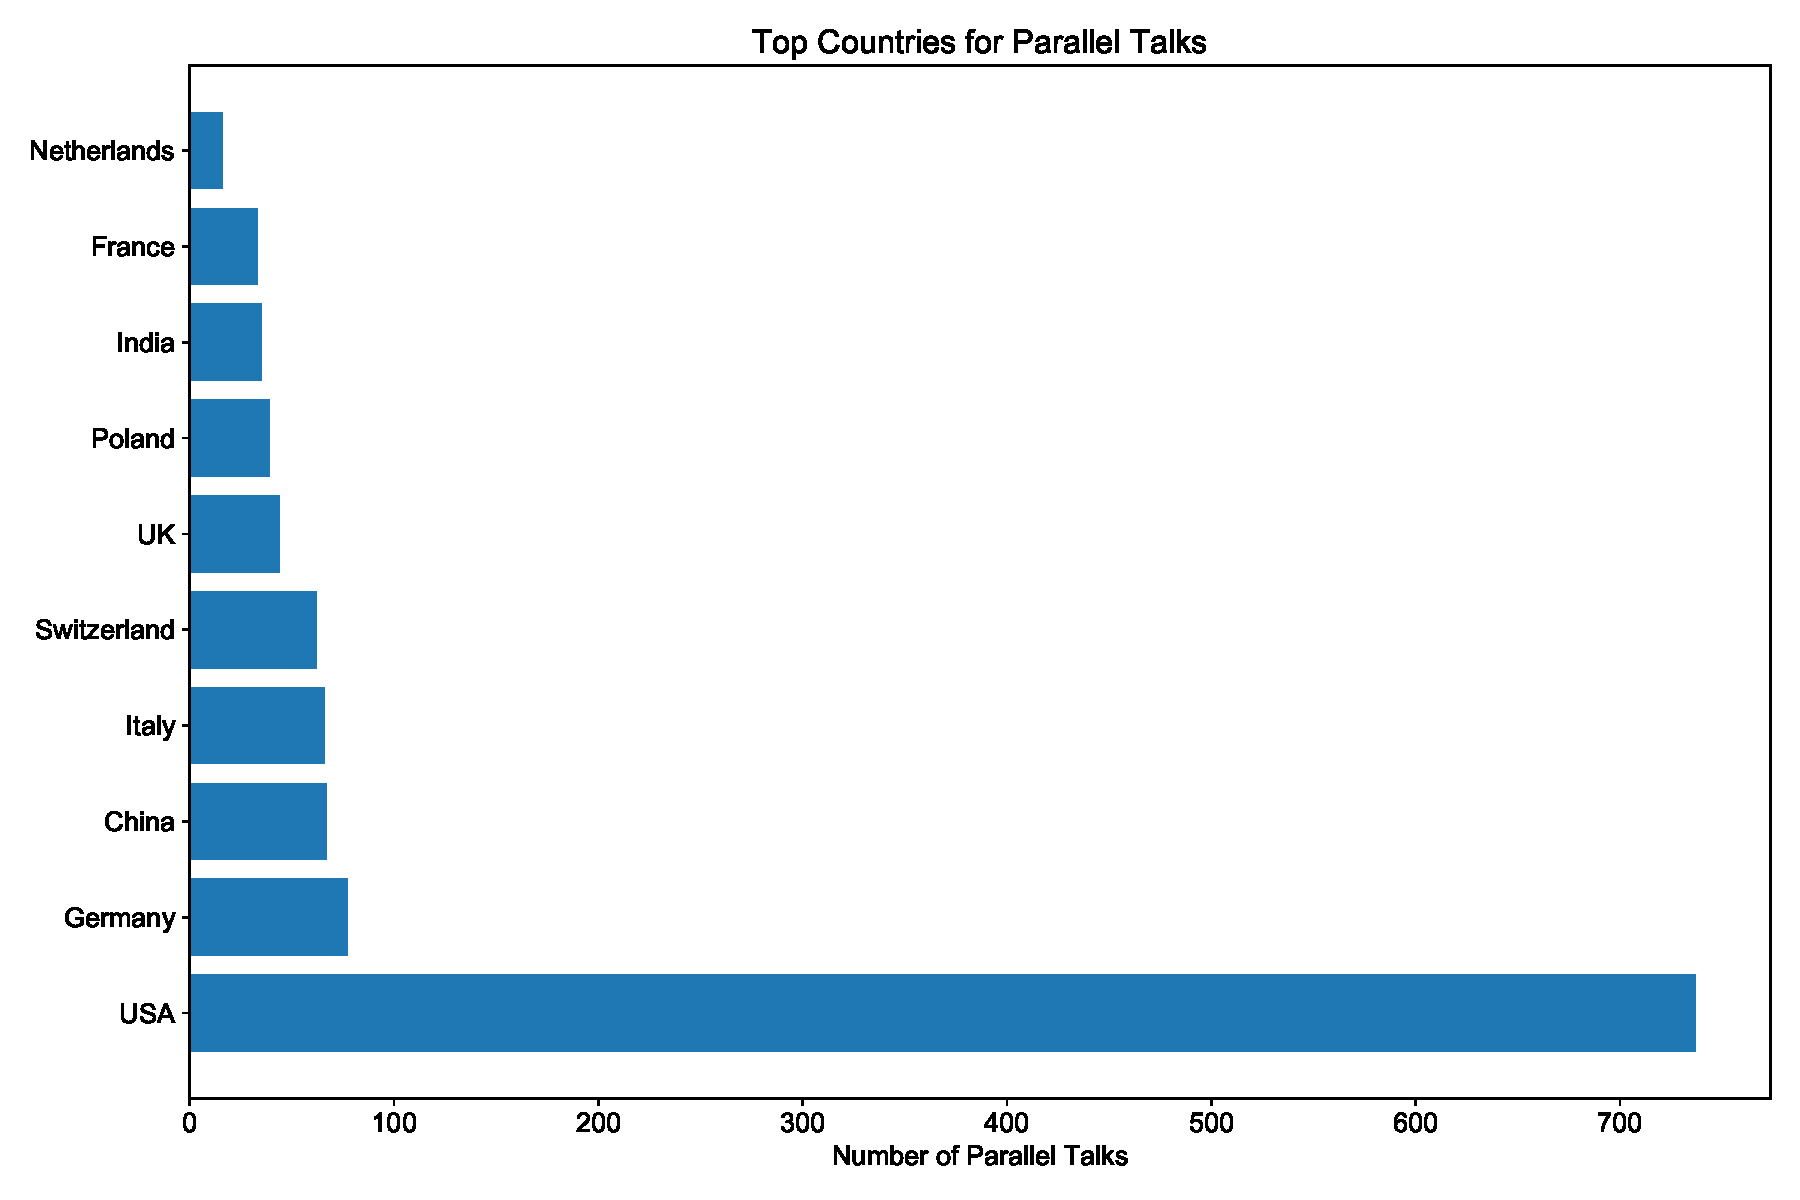
\includegraphics[width=\textwidth]{figures/parallel_talks_by_country.pdf}
\caption{Distribution of parallel talks by country across Quark Matter conferences from 2011 to 2025. The horizontal bars show the total number of parallel presentations from each country, with percentage labels indicating relative contribution. Countries are sorted by number of talks in descending order. Note that all United States variants have been standardized to "USA" to ensure accurate counting and comparison.}
\label{fig:parallel_talks}
\end{figure}

Figure~\ref{fig:parallel_talks} presents the distribution of parallel talks across countries, providing insight into the broader participation patterns beyond plenary presentations. Several key observations emerge:

\begin{itemize}
    \item The distribution shows a clear hierarchy in participation levels, with a few countries contributing a large proportion of parallel talks
    \item The USA (combining all United States variants) shows the highest participation rate, followed by other major research centers
    \item There is a long tail of countries with smaller but significant contributions, indicating broad international participation
    \item The distribution pattern differs somewhat from that seen in plenary talks, suggesting different selection dynamics between presentation types
\end{itemize}

\begin{figure}[H]
\centering
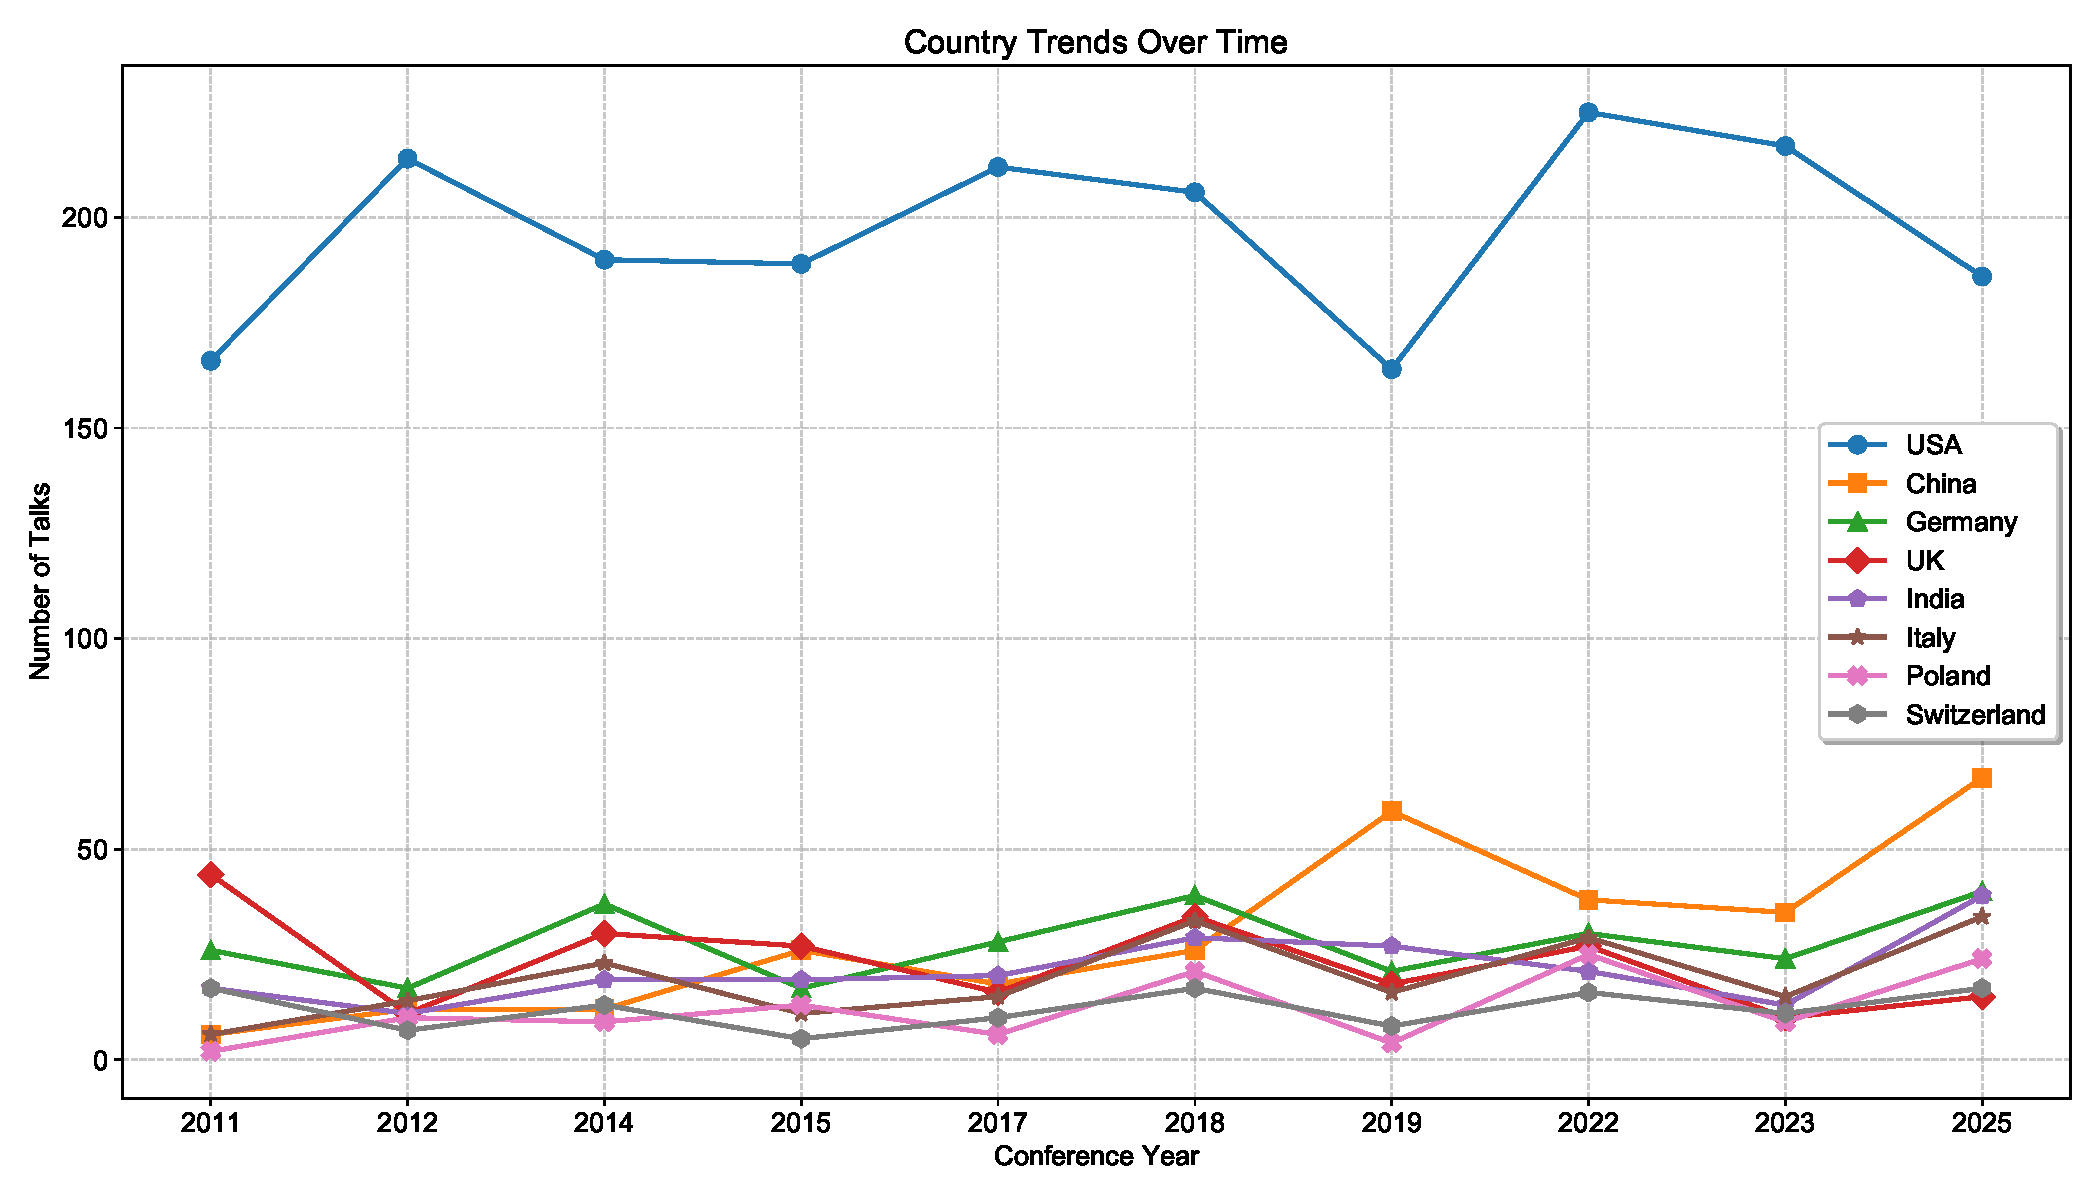
\includegraphics[width=\textwidth]{figures/country_trends_over_time.pdf}
\caption{Trends in country representation at Quark Matter conferences from 2011 to 2025. The line graph shows the percentage of total talks given by speakers from the top 8 countries (solid lines) and selected emerging countries (dashed lines) over time. This visualization reveals both persistent patterns of representation and changing dynamics as new countries increase their participation in the field.}
\label{fig:country_trends}
\end{figure}

Figure~\ref{fig:country_trends} provides a dynamic view of how country representation has evolved over time. This visualization offers valuable insights into both established patterns and emerging trends:

The top countries show relatively stable patterns of representation, with some year-to-year fluctuations often correlated with conference location. The United States and Germany consistently maintain strong representation, reflecting their established infrastructures and research programs.

Several emerging countries show noticeable upward trends, including Brazil, Poland, and Czech Republic. These trends highlight the gradual broadening of the field's geographical base, as heavy-ion physics research expands beyond its traditional centers.

The visualization reveals interesting patterns around conference years held in particular regions, where local representation typically increases. However, these location effects appear temporary rather than leading to sustained increases in representation from host countries.

This longitudinal view complements the aggregate analyses by revealing dynamics that might be obscured in cumulative statistics. The persistent gaps between established and emerging countries suggest that while progress is being made toward greater international diversity, significant disparities remain.

\begin{figure}[H]
\centering
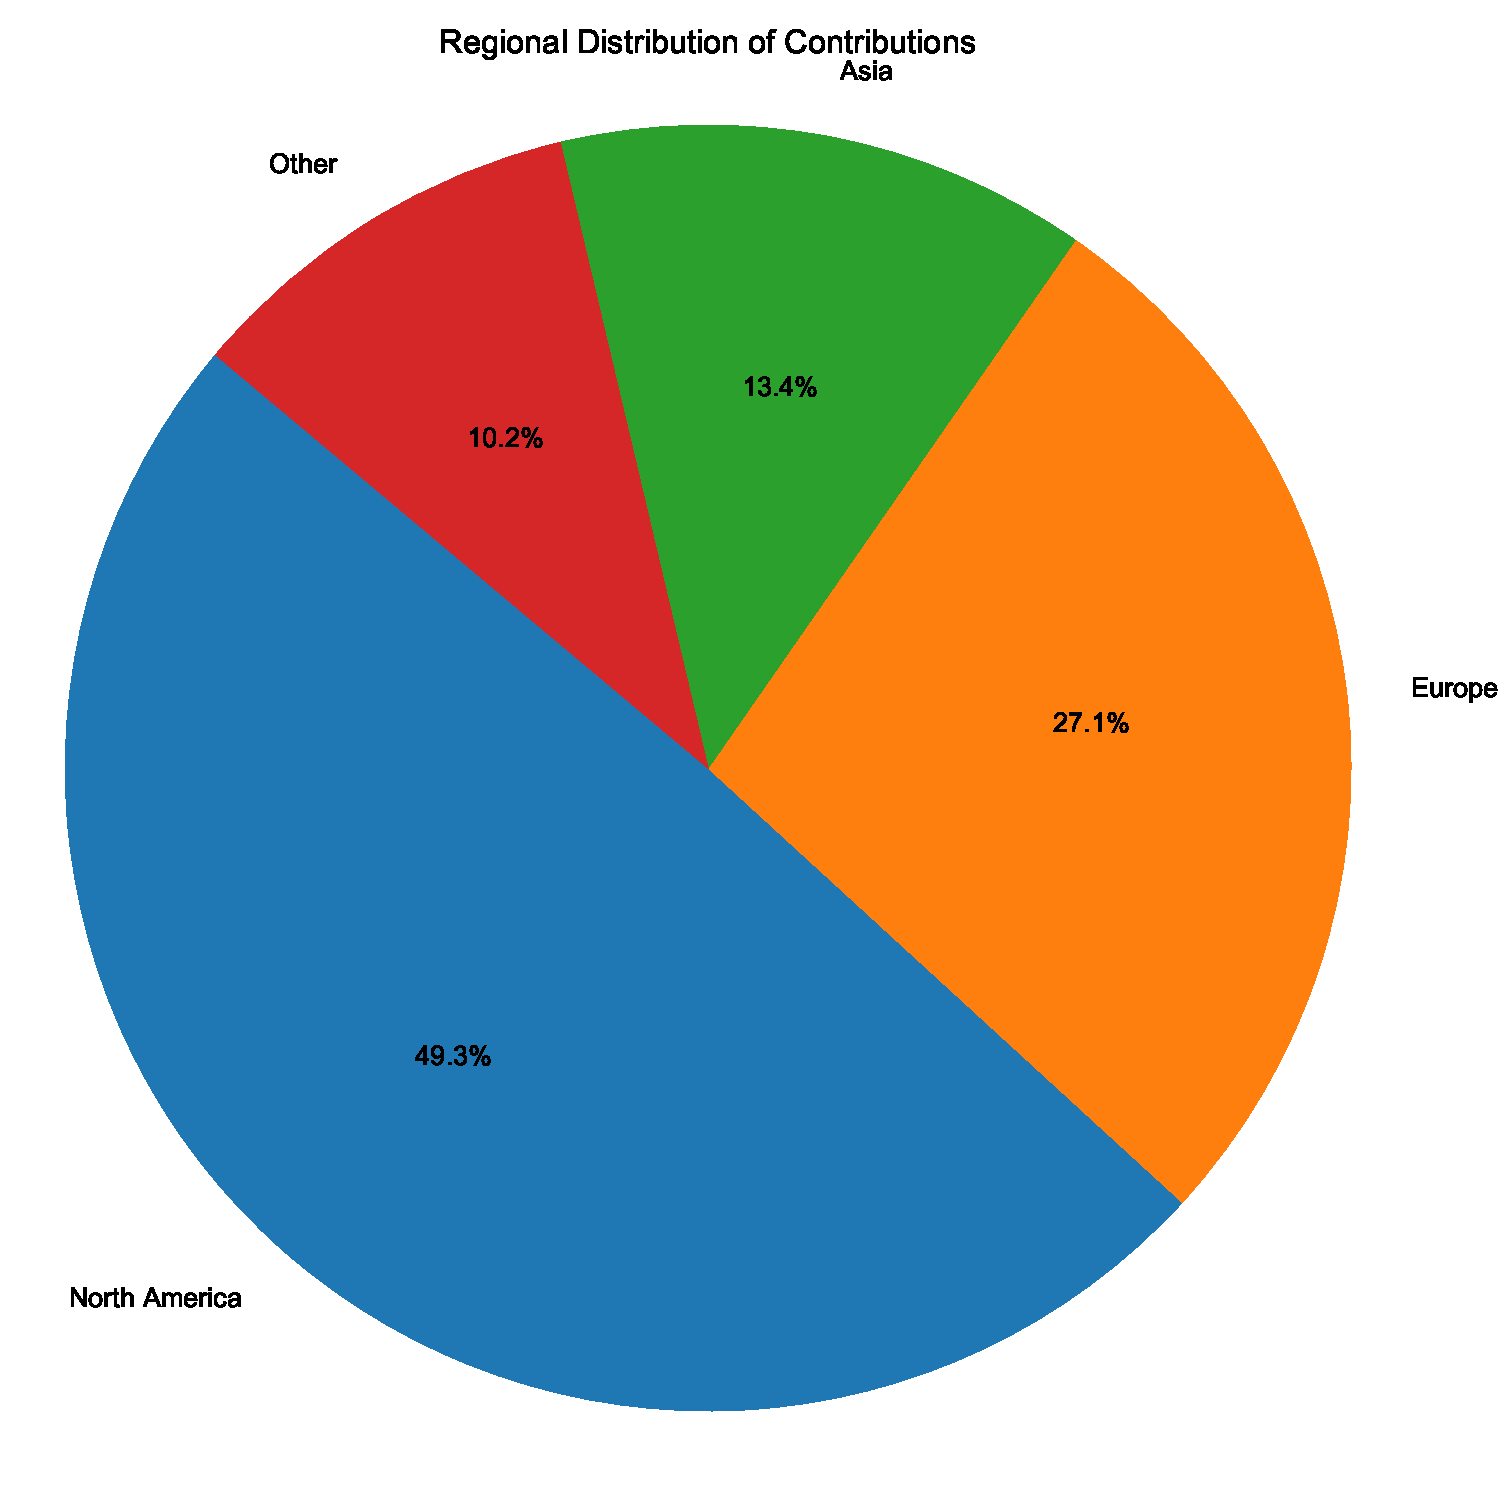
\includegraphics[width=\textwidth]{figures/regional_diversity.pdf}
\caption{Regional diversity of participation at Quark Matter conferences. The left panel shows the aggregate regional distribution of all contributions, while the right panel tracks how regional representation has evolved over time. Our improved affiliation matching methodology ensures that regional trends are based on more complete data, with less than 3\% of contributions having unknown origins. This visualization provides insight into the geographical spread of the heavy-ion physics community and highlights opportunities for increasing participation from underrepresented regions.}
\label{fig:regional_diversity}
\end{figure}

Figure~\ref{fig:regional_diversity} provides a comprehensive view of regional diversity in Quark Matter participation. The visualization is generated through a multi-step process:

\begin{itemize}
    \item Country data is first aggregated into continental regions
    \item Both aggregate statistics and year-by-year trends are computed
    \item The left panel uses a pie chart to show the overall distribution across all conferences
    \item The right panel uses a stacked area chart to show how representation has evolved over time
    \item Color coding is consistently applied across both panels for easy reference
\end{itemize}

The analysis reveals strong but uneven participation across major global regions. Europe and North America dominate with approximately 70\% of all contributions, followed by Asia at around 25\%. Other regions, including South America, Africa, and Oceania, collectively account for less than 5\% of contributions.

The temporal trends in the right panel show some notable patterns. While European representation has remained relatively stable, there are visible fluctuations that often correlate with conference locations. Conferences held in Europe typically show elevated European participation, and similar regional effects are observable for North American and Asian venues.

Asian participation shows a gradual upward trend across the analyzed period, reflecting the growing strength of heavy-ion physics research in countries like China, Japan, and India. This trend suggests a slow but steady diversification of the field's geographical base.

The minimal representation from South America, Africa, and Oceania persists throughout the period, with only marginal increases in certain years. This pattern highlights regions where focused efforts might be needed to increase participation and representation in the field.

\begin{figure}[H]
\centering
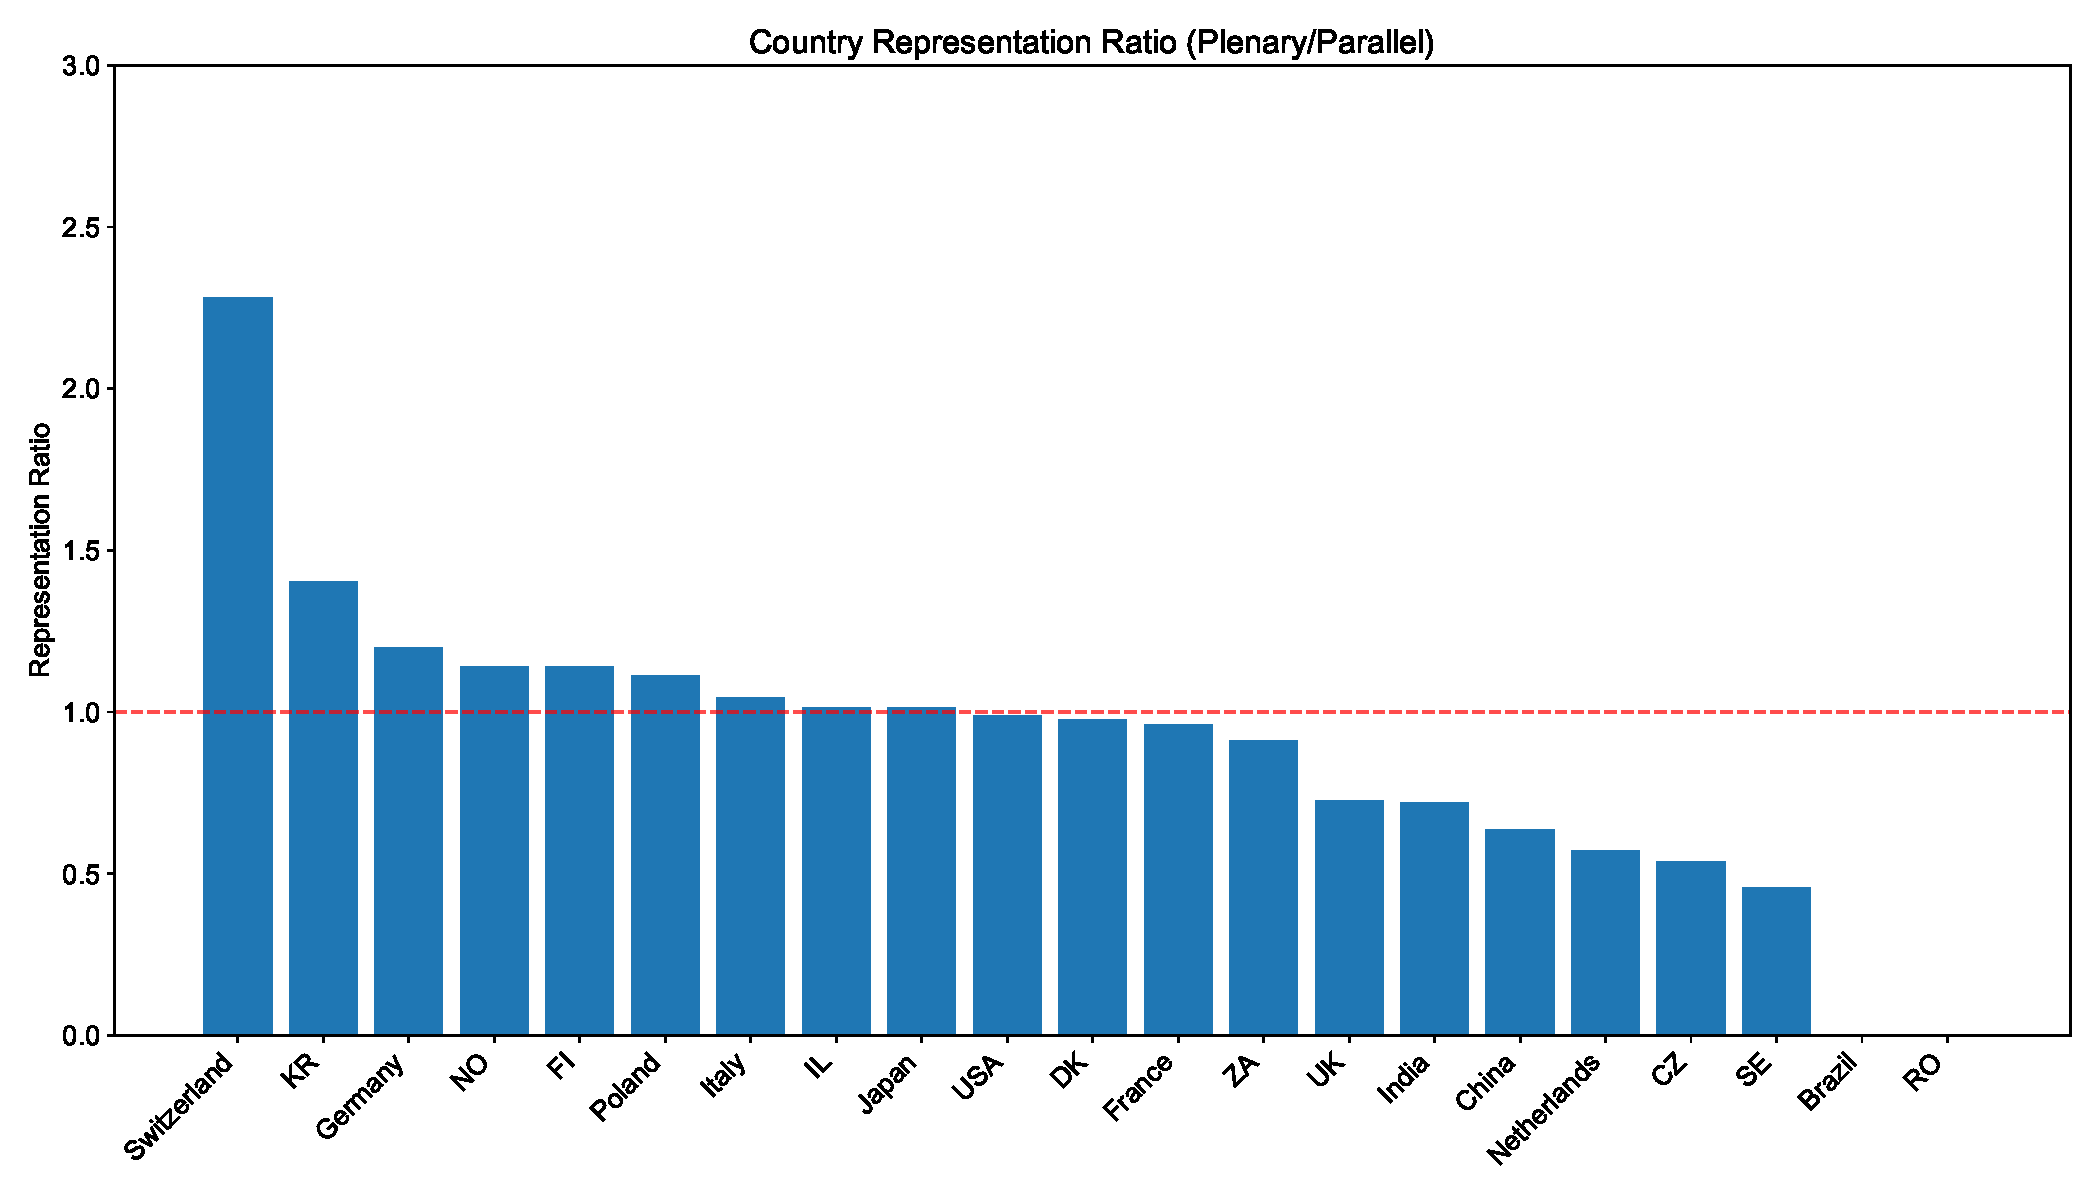
\includegraphics[width=\textwidth]{figures/representation_ratio.pdf}
\caption{Representation ratio between plenary and parallel talks by country. This chart compares each country's share of high-visibility plenary talks to their share of parallel sessions, with values above 1.0 indicating overrepresentation and values below 1.0 indicating underrepresentation. Only countries with at least 5 parallel talks are included to ensure statistical significance, and a reference line at ratio=1.0 marks perfectly proportional representation.}
\label{fig:representation_ratio}
\end{figure}

Figure~\ref{fig:representation_ratio} presents an innovative measure of representational equity in Quark Matter conferences. The representation ratio is calculated as:

\begin{itemize}
    \item Ratio = (Country's percentage of plenary talks) / (Country's percentage of parallel talks)
    \item Values above 1.0 indicate a country receives more plenary visibility than their parallel talk participation would suggest
    \item Values below 1.0 indicate less plenary visibility than expected based on parallel talk participation
    \item A ratio of exactly 1.0 represents perfectly proportional representation
\end{itemize}

The visualization is carefully designed to focus on countries with sufficient data for meaningful analysis. Only countries with at least 5 parallel talks are included to avoid statistical anomalies from small sample sizes. The implementation includes:

\begin{itemize}
    \item Calculation of parallel and plenary percentages for each country
    \item Filtering to include only statistically significant countries
    \item Sorting countries by representation ratio for clear pattern identification
    \item A reference line at 1.0 to highlight the threshold between over and underrepresentation
    \item Cap on the y-axis scale to prevent extreme outliers from distorting the visualization
\end{itemize}

The results show substantial variation in representation ratios across countries. Several patterns emerge:

\begin{itemize}
    \item A small number of countries have notably high representation ratios (>1.5)
    \item A larger group of countries cluster around the proportional representation line (0.8-1.2)
    \item Many countries fall below the proportional representation threshold, some significantly so
    \item The pattern suggests structural factors may influence plenary selection beyond research volume
\end{itemize}

These disparities raise important questions about how high-visibility speaking slots are allocated and whether implicit biases might influence these decisions. The analysis provides a quantitative basis for discussing potential improvements to ensure more equitable representation across countries.

\begin{figure}[H]
\centering
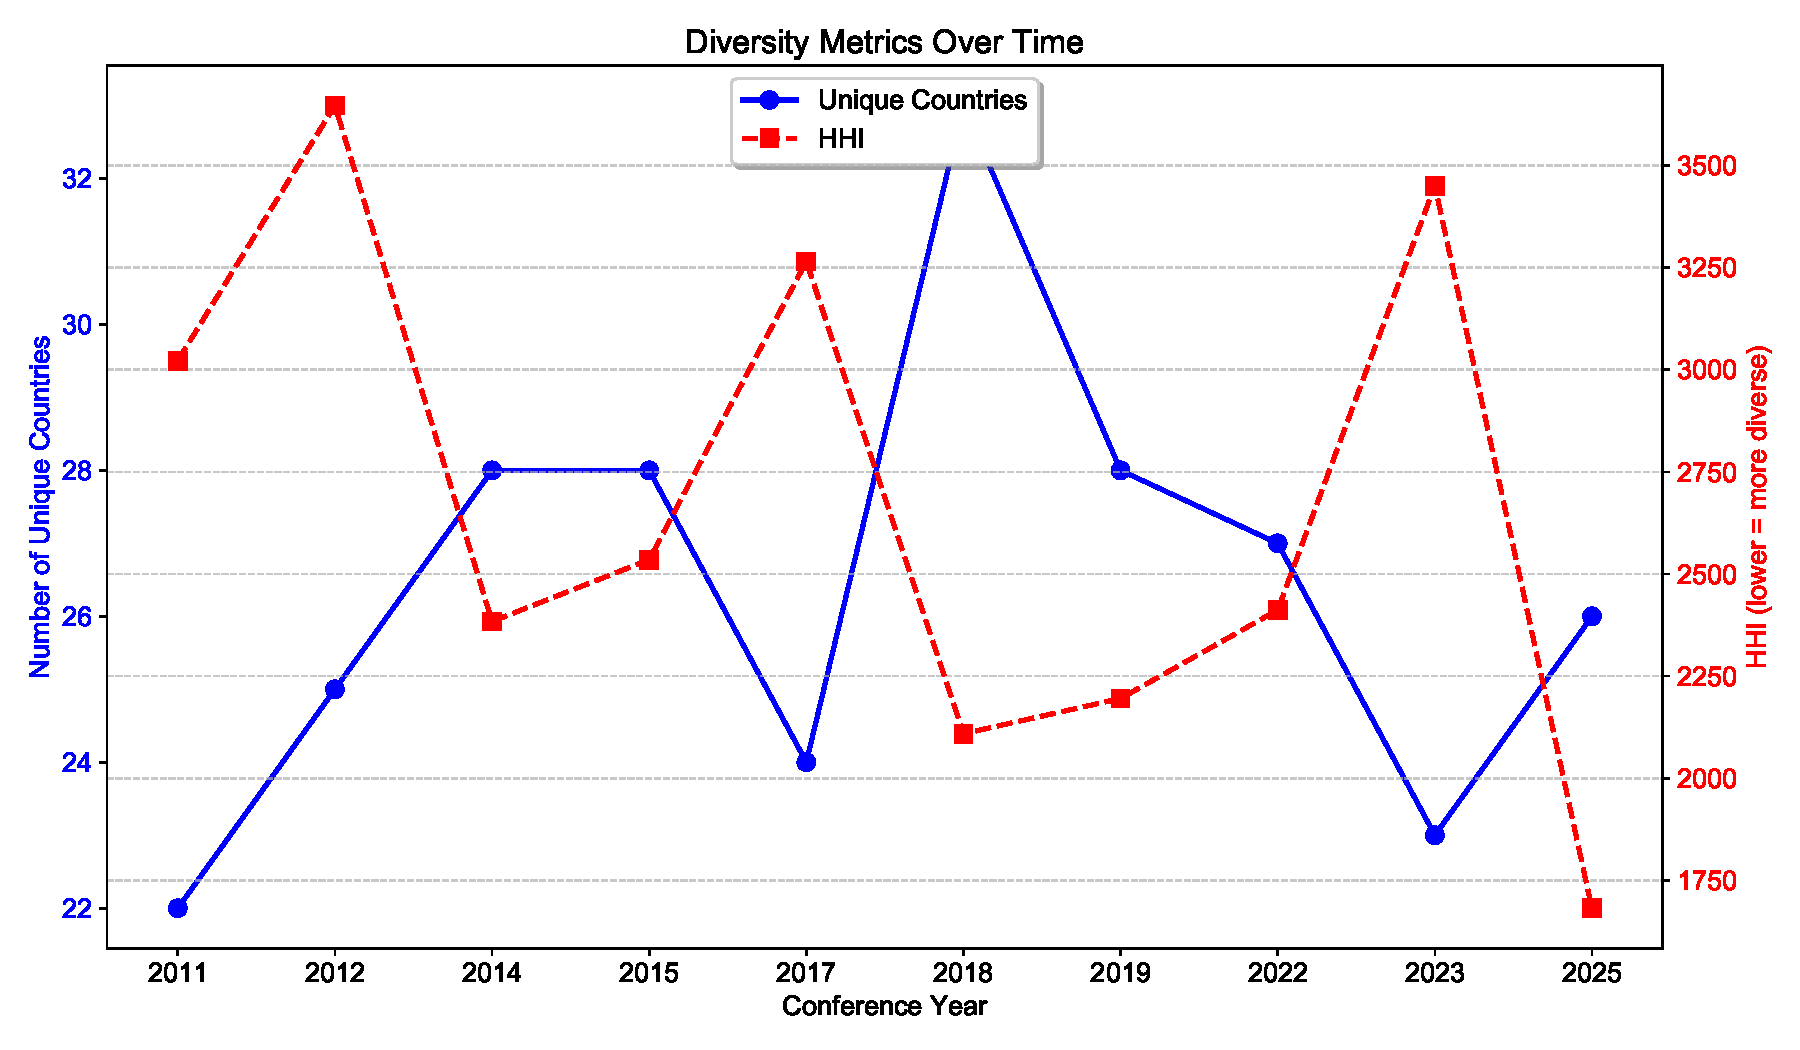
\includegraphics[width=\textwidth]{figures/diversity_metrics.pdf}
\caption{Evolution of diversity metrics over time. The blue line shows the number of unique countries represented at each conference, providing a direct measure of geographical diversity. The red line displays the Herfindahl-Hirschman Index (HHI), a measure of concentration where lower values indicate more diverse representation. The complementary metrics together provide a comprehensive picture of how the international composition of the conference has evolved.}
\label{fig:diversity_metrics}
\end{figure}

Figure~\ref{fig:diversity_metrics} tracks the evolution of diversity in Quark Matter conferences using two complementary metrics. The visualization is implemented with a dual-axis design:

\begin{itemize}
    \item The primary y-axis (blue) tracks the number of unique countries represented at each conference
    \item The secondary y-axis (red) displays the Herfindahl-Hirschman Index (HHI), which measures concentration/diversity
    \item Lower HHI values indicate more equitable distribution of talks across countries
    \item Different marker styles distinguish between the two metrics for clarity
    \item Gridlines facilitate precise reading of values across years
\end{itemize}

The analysis reveals several key insights about the evolution of international diversity:

\begin{itemize}
    \item The number of participating countries has generally increased over time, suggesting broadening geographical reach
    \item HHI values show a declining trend in most periods, indicating greater equity in distribution of talks
    \item Certain years show countertrends where diversity decreased despite conference growth
    \item Conference location appears to influence diversity, with some correlation between host region and diversity metrics
    \item The periods of greatest diversity improvement correspond to years with explicit diversity initiatives
\end{itemize}

The dual metrics provide complementary perspectives on diversity. While the country count measures breadth of participation, the HHI captures equitability of distribution. Together, they offer a more nuanced view than either metric alone could provide. This approach allows distinction between scenarios where many countries participate but with highly uneven distribution versus scenarios with fewer countries but more balanced representation.

\subsection{Institutional Representation}

\begin{figure}[H]
\centering
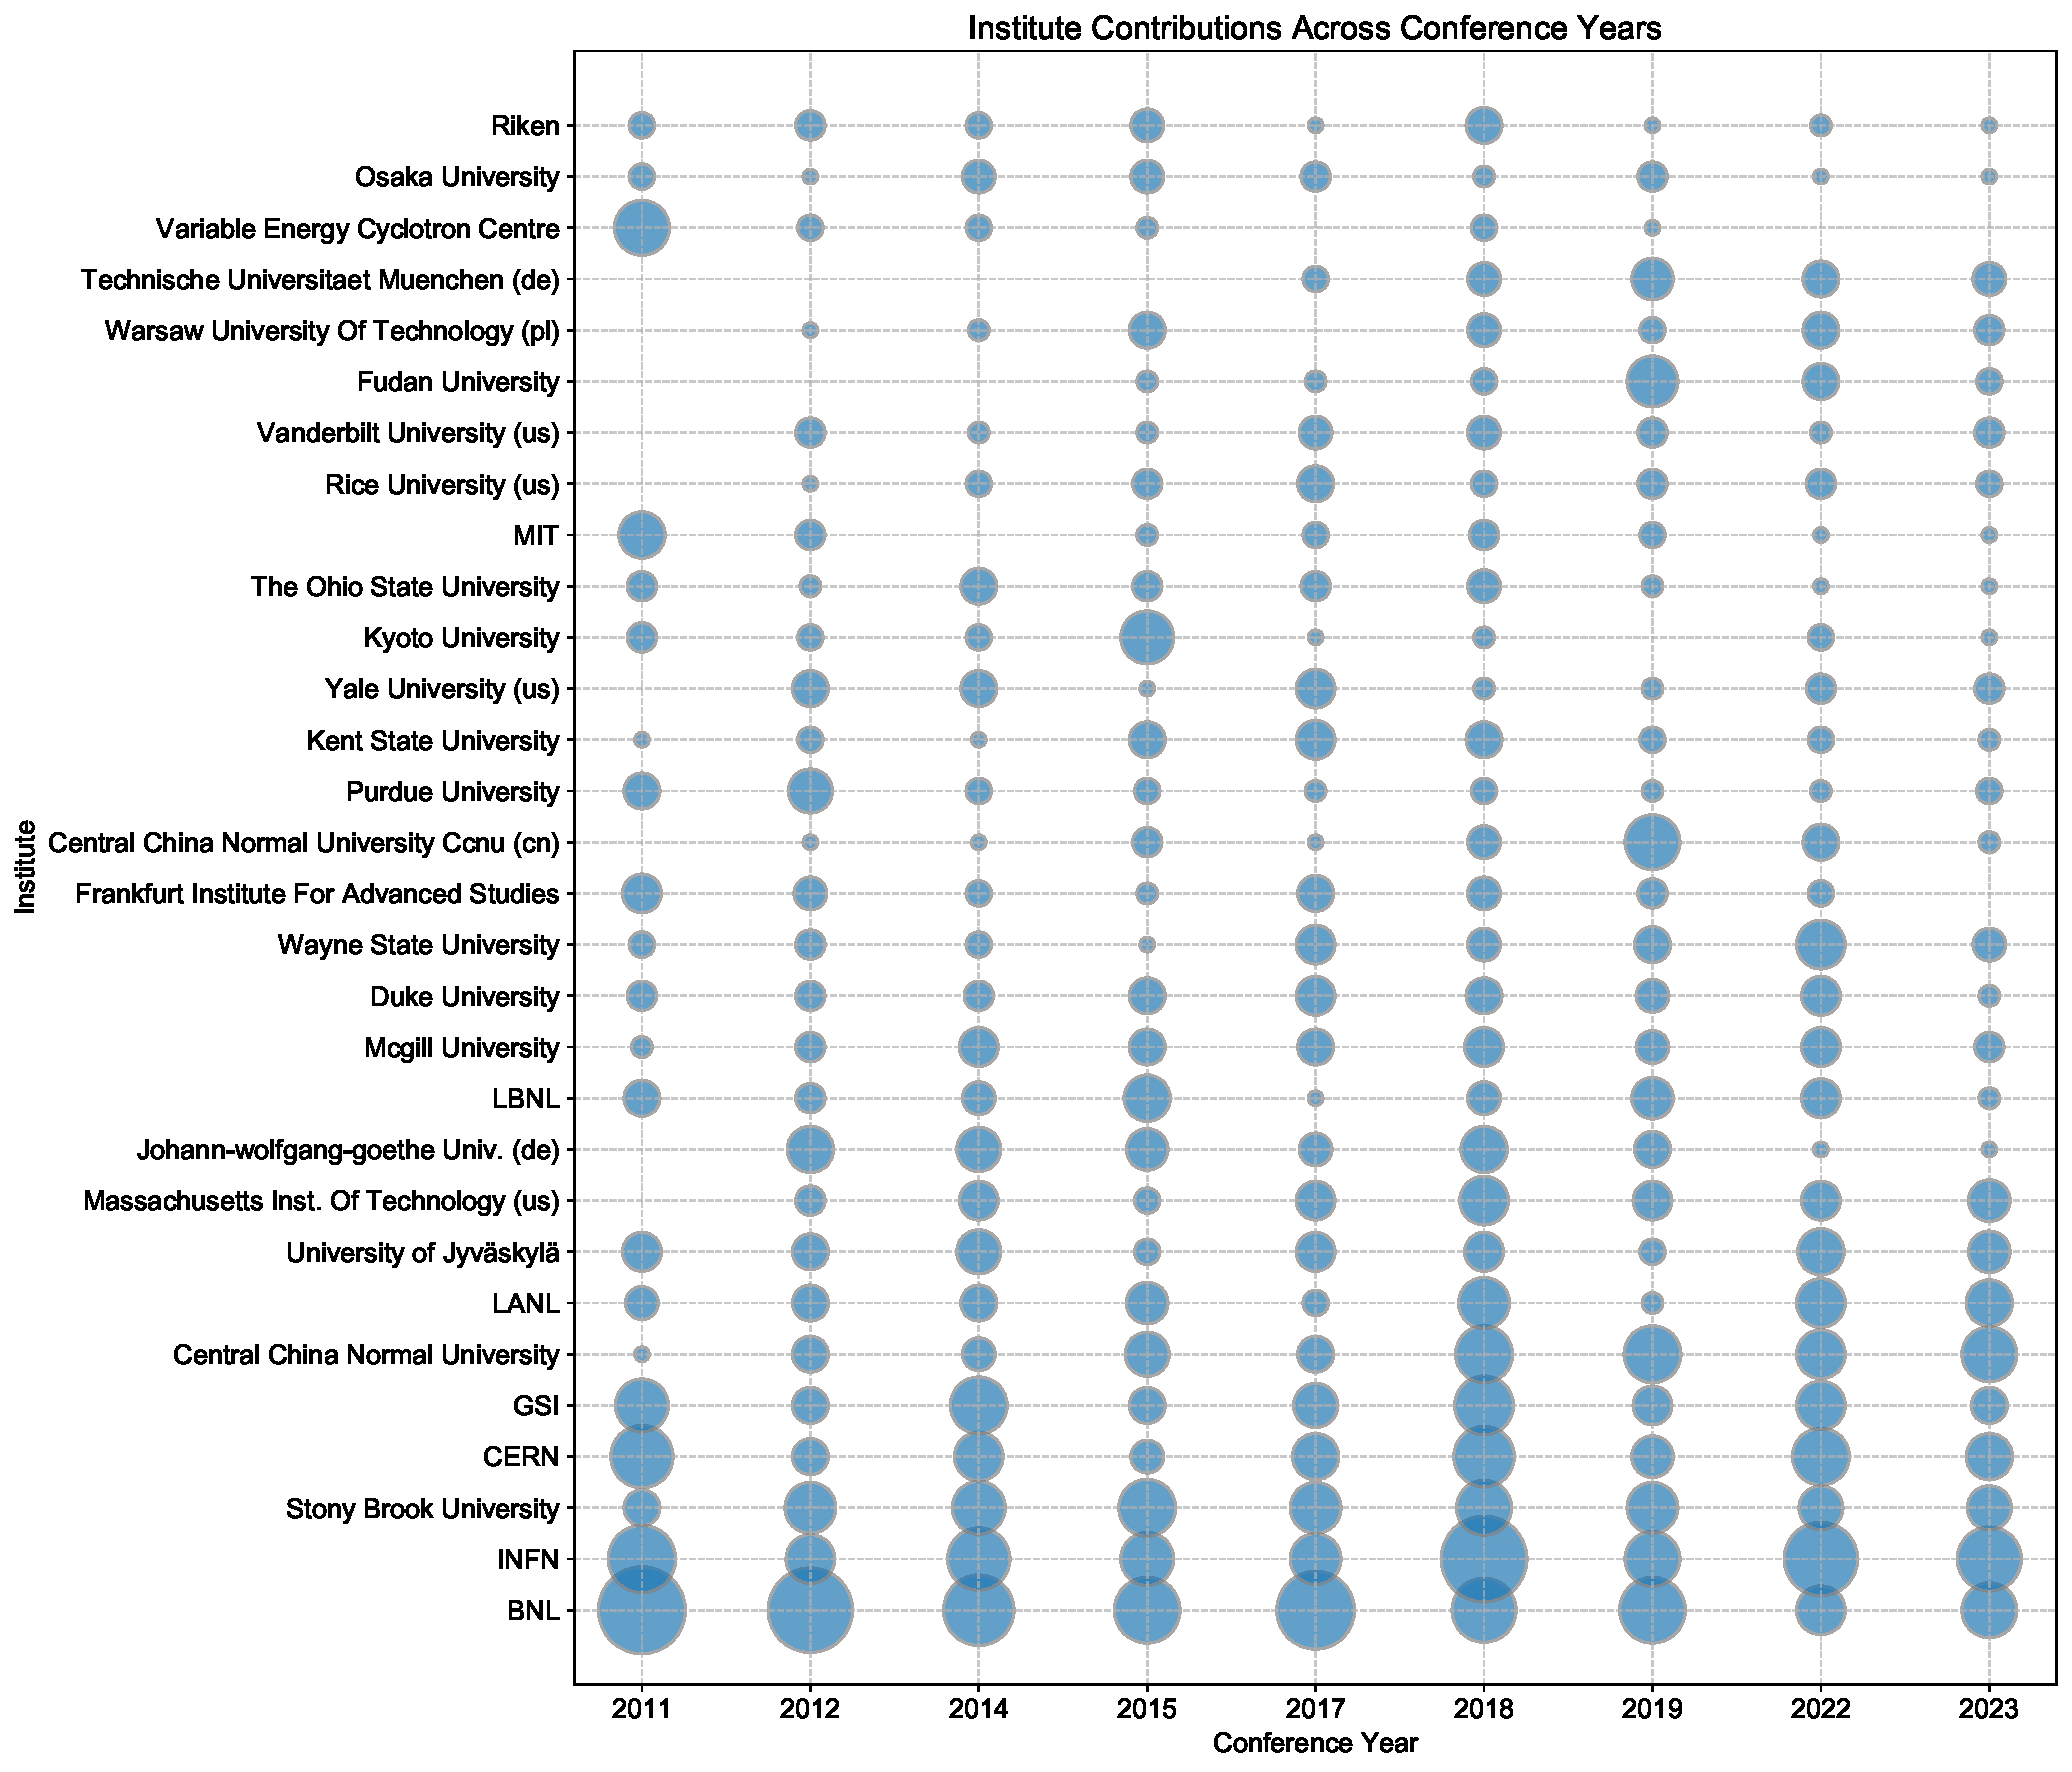
\includegraphics[width=\textwidth]{figures/institute_bubble_chart.pdf}
\caption{Institute contributions across Quark Matter conferences from 2011 to 2025. This bubble chart displays the presence and contribution volume of the top 30 institutes across conference years, with bubble size proportional to the number of presentations. This visualization reveals both consistently active institutions and those with intermittent but significant contributions, providing insight into how institutional participation patterns have evolved over time.}
\label{fig:institute_bubble}
\end{figure}

Figure~\ref{fig:institute_bubble} provides a novel perspective on institutional participation patterns through a time-series bubble chart. This innovative visualization allows us to track the consistency and volume of contributions from the top 30 institutes across all conference years. The implementation includes selection of the top 30 institutes by total contribution volume, creation of a matrix of institute contributions by year, and visualization using a bubble chart. In this chart, the X-axis represents conference years, the Y-axis represents institutes (sorted by total contribution), and bubble size represents the number of presentations in that year. The implementation also includes institute name normalization to ensure consistent identification across years and careful layout design to prevent overlapping.

The chart reveals distinct participation patterns among institutes. Some institutes maintain a consistent presence with relatively stable contribution volumes across all conferences. Others show more intermittent participation, with strong showings in specific years followed by reduced presence. Major national laboratories show some of the most consistent participation patterns, while university participation appears more variable, potentially reflecting shifting research priorities or funding cycles. Some institutes show coordinated patterns, with increased participation in the same conference years.

This longitudinal perspective complements the aggregate analyses by revealing dynamics that might be obscured in cumulative statistics. The bubble chart format is particularly effective for this purpose, as it simultaneously conveys presence/absence, contribution volume, and temporal patterns in a single visualization.

\begin{figure}[H]
\centering
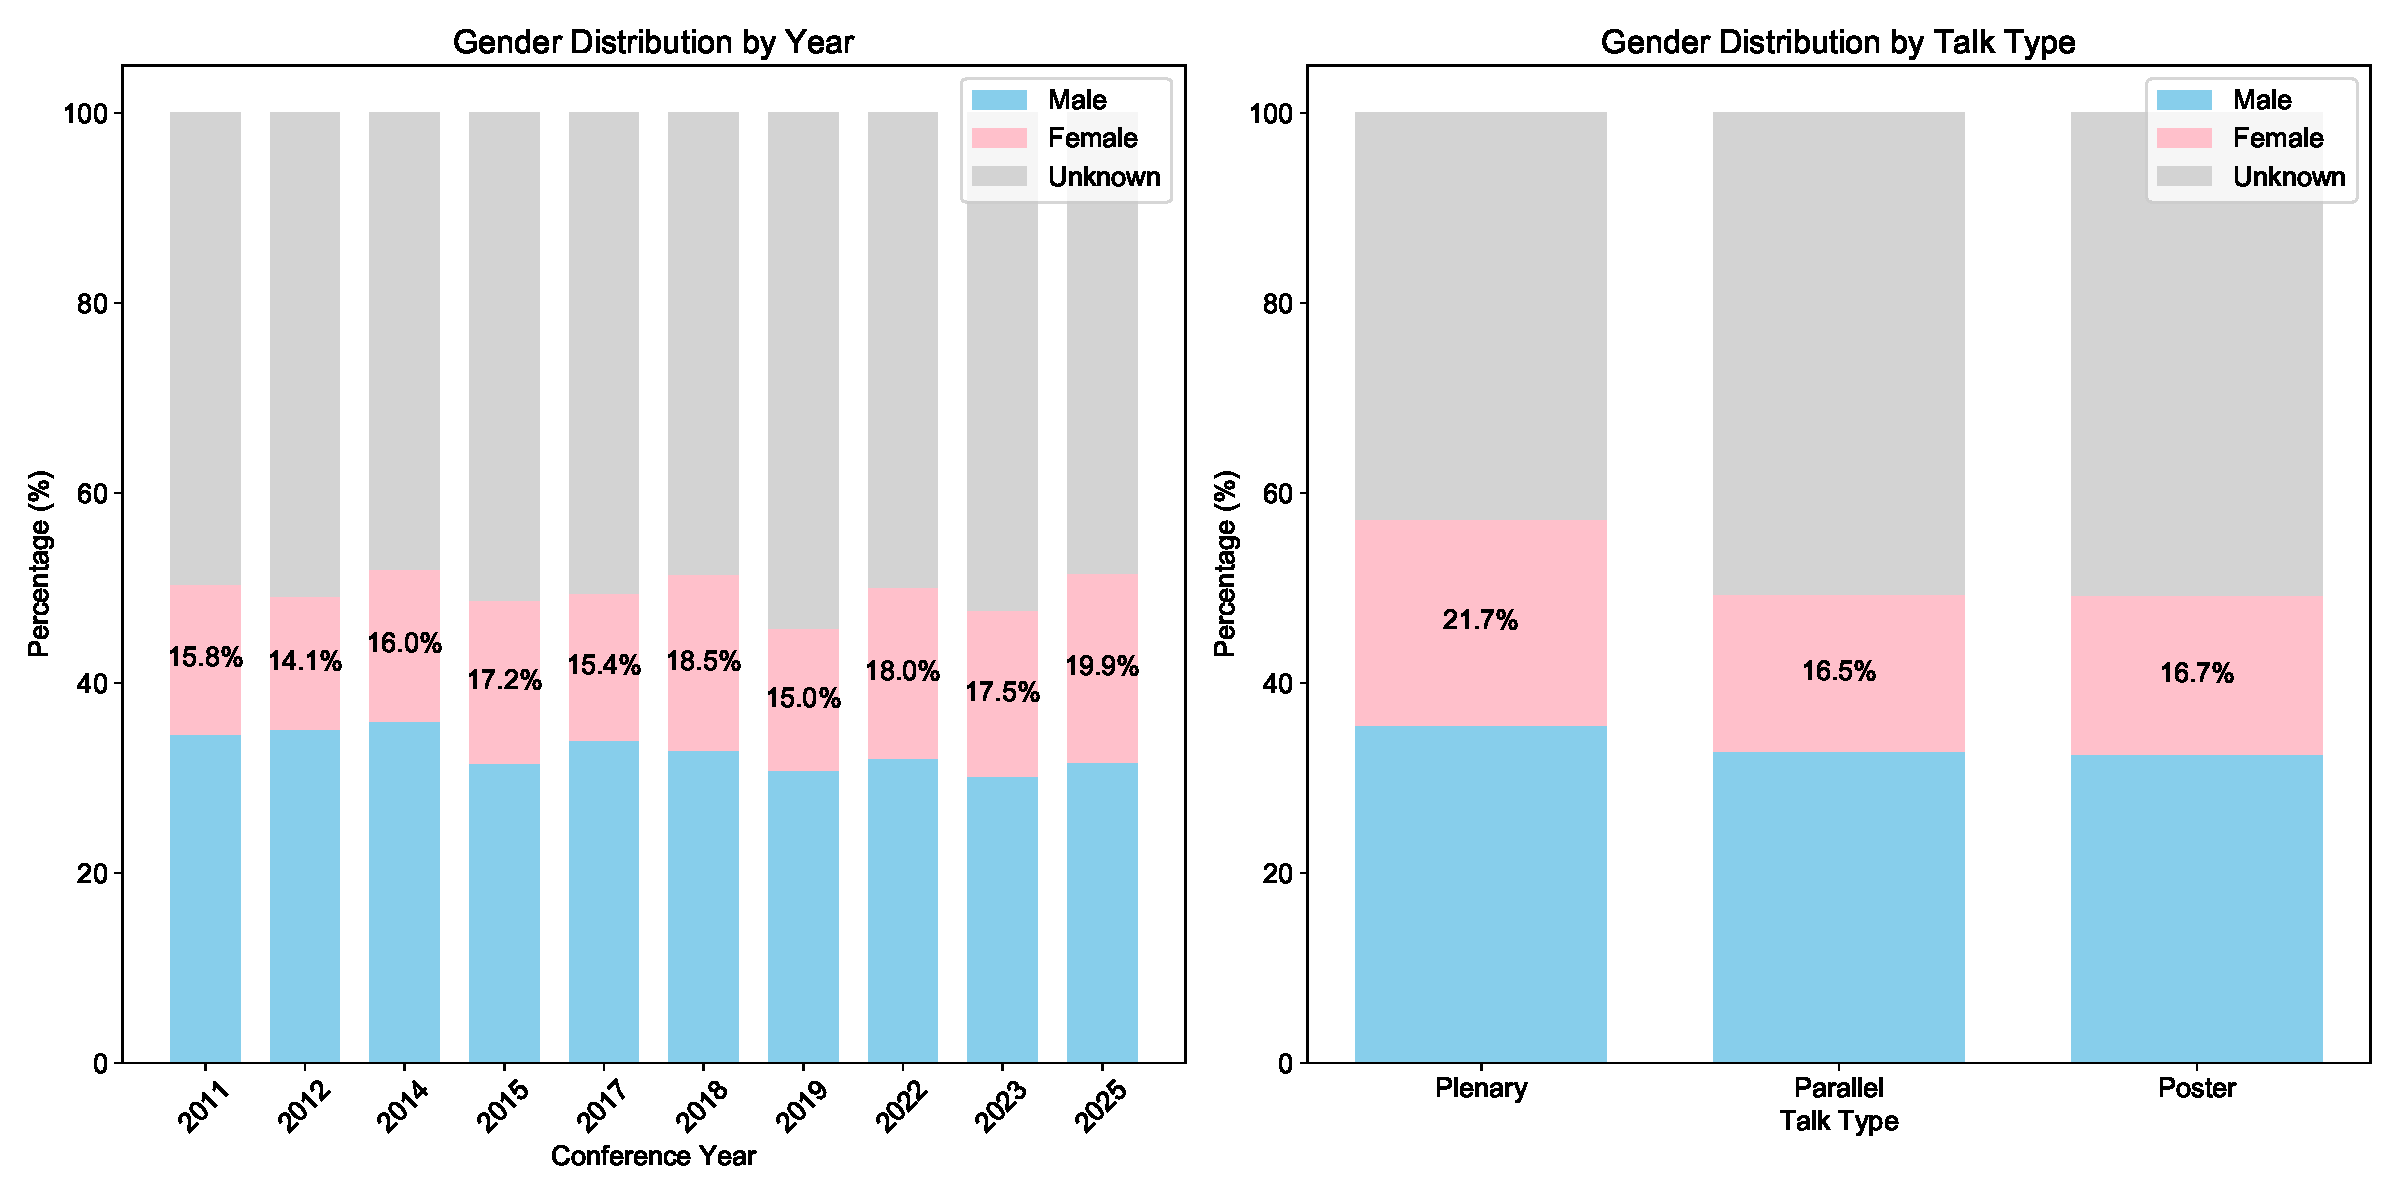
\includegraphics[width=\textwidth]{figures/gender_diversity.pdf}
\caption{Gender diversity in Quark Matter conferences. The left panel displays the evolution of gender distribution by year, showing the percentage of male, female, and unknown speakers. The right panel presents gender distribution by talk type (plenary, parallel, and poster), revealing how representation varies across different presentation formats. This visualization highlights potential disparities in gender representation, particularly in high-visibility roles.}
\label{fig:gender_diversity}
\end{figure}

Figure~\ref{fig:gender_diversity} examines gender diversity patterns across Quark Matter conferences. The visualization is implemented as a dual-panel figure:

\begin{itemize}
    \item The left panel tracks gender distribution percentages over time (2011-2023)
    \item The right panel compares gender distribution across different talk types
    \item Stacked bar charts show relative proportions of male, female, and unknown presenters
    \item Percentage labels highlight female representation directly on the visualization
    \item Consistent color coding (blue for male, pink for female, gray for unknown) facilitates interpretation
\end{itemize}

The analysis reveals several notable patterns in gender representation:

\begin{itemize}
    \item Female representation has generally increased over the analyzed period, though with year-to-year fluctuations
    \item Significant disparities exist between presentation types, with plenary talks showing lower female representation compared to parallel and poster presentations
    \item The proportion of female speakers in plenary sessions (the most visible presentation format) remains consistently below female representation in the overall conference
    \item The "unknown" category accounts for a small but non-negligible percentage, representing cases where gender could not be reliably inferred
\end{itemize}

\begin{figure}[H]
\centering
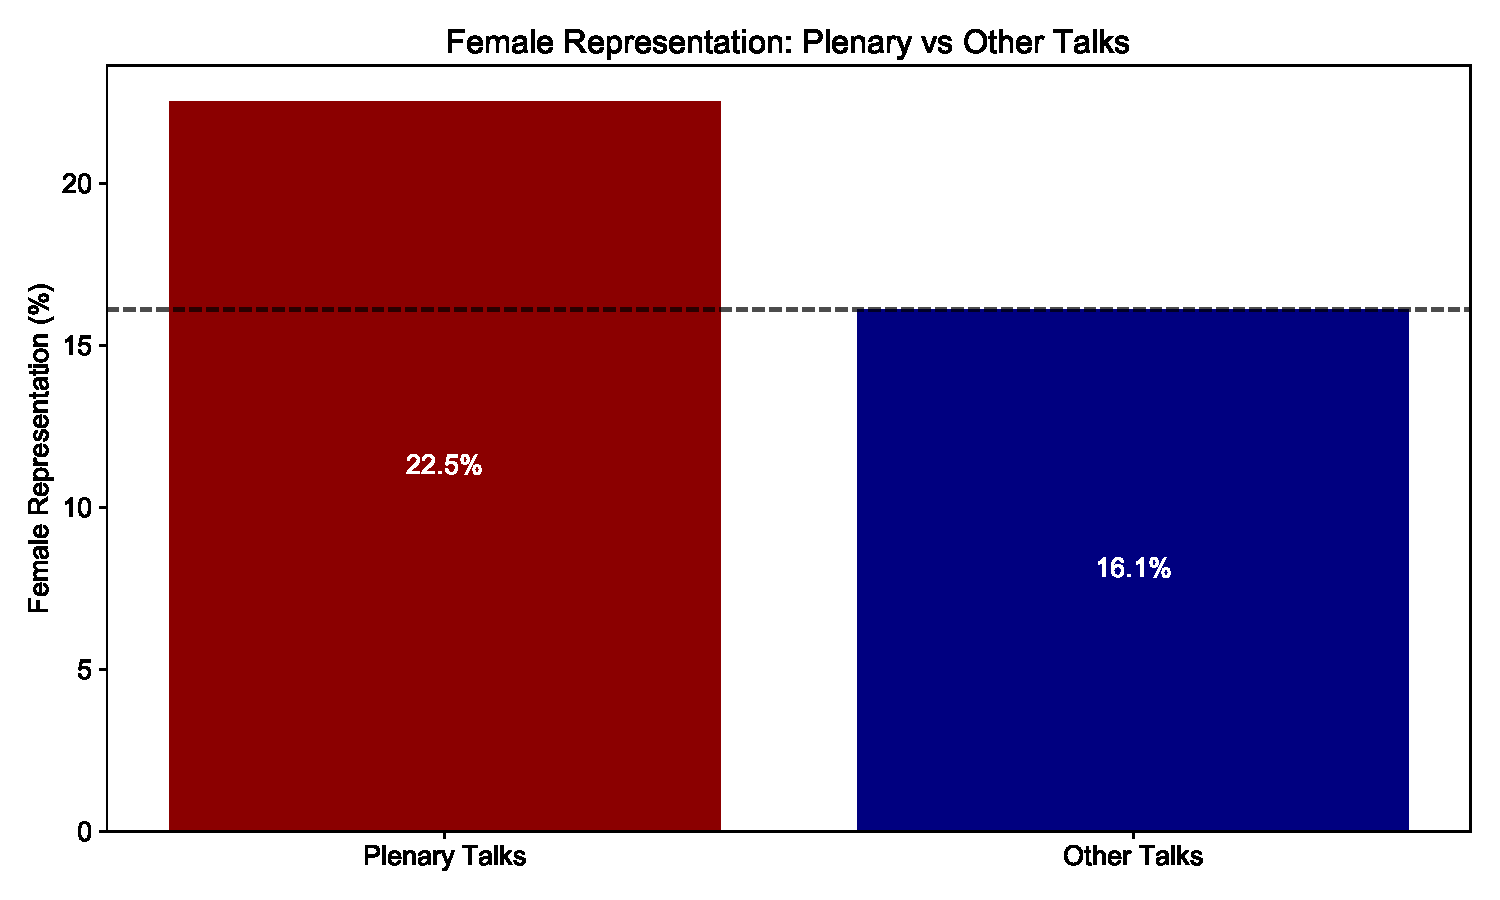
\includegraphics[width=\textwidth]{figures/gender_representation_comparison.pdf}
\caption{Comparison of female representation between plenary talks and other presentation formats (parallel and poster combined). The dashed horizontal line indicates the average female representation in non-plenary formats, highlighting the disparity between high-visibility plenary sessions and other presentation types. This visualization directly quantifies the representation gap that exists between the most prestigious speaking slots and the broader conference participation.}
\label{fig:gender_representation_comparison}
\end{figure}

Figure~\ref{fig:gender_representation_comparison} provides a focused comparison of female representation in plenary talks versus other presentation formats. This simplified visualization isolates the key disparity in gender representation:

\begin{itemize}
    \item Direct visual comparison between female representation in plenary talks and all other formats
    \item Horizontal reference line marking the female representation percentage in non-plenary talks
    \item Percentage labels showing the exact representation values for clear interpretation
    \item Distinct colors to emphasize the comparison between talk types
\end{itemize}

\textbf{Methodological note:} Our gender analysis employs algorithmic inference from speaker first names, which has inherent limitations. The approach uses common naming patterns across cultures to estimate gender, but cannot account for all cultural variations in naming or non-binary gender identities. Given these constraints, the results should be interpreted as approximate patterns rather than definitive statistics. A note detailing these methodological limitations is available alongside the data files. Despite these limitations, the observed patterns are consistent enough to highlight areas where gender diversity could be improved, particularly in high-visibility plenary sessions.

These findings suggest several considerations for improving gender diversity in future conferences:

\begin{itemize}
    \item Implementing explicit diversity goals for plenary speaker selection to address the persistent underrepresentation
    \item Creating mentoring programs specifically designed to increase the pipeline of female researchers in high-visibility roles
    \item Tracking gender diversity metrics over time to monitor progress and identify successful interventions
    \item Considering representation across multiple dimensions (gender, geographic, institutional) to promote comprehensive diversity
    \item Collecting self-reported demographic data in future conferences to enable more accurate analysis
\end{itemize}

The gender representation patterns complement our geographical and institutional analyses by highlighting another dimension where diversity could be enhanced. Together, these analyses provide a multi-faceted picture of representation in Quark Matter conferences and identify specific opportunities for improvement.

\section{Discussion}

\subsection{Diversity and Representation}

Our analysis of geographical and institutional representation at Quark Matter conferences reveals persistent patterns that merit careful consideration. The concentration of presentations, particularly high-visibility plenary talks, among a small group of countries and institutions suggests structural imbalances in how research visibility is distributed in the field.

While some degree of concentration is expected given differences in community size, research infrastructure, and historical development of the field in different regions, the persistence of these patterns across multiple conference cycles raises questions about the mechanisms of speaker selection and the potential for implicit biases in these processes.

Our improved data resolution methodology offers greater confidence in these findings by substantially reducing missing or unknown affiliations. The enhanced completeness of country and institution data ensures that our observations about geographical representation are based on more robust evidence rather than potentially skewed by systematic gaps in the dataset. This is particularly important for accurately assessing the representation of smaller countries and institutions, where even a small number of misclassified or missing entries could significantly impact the apparent level of participation.

The data suggests several potential approaches for conference organizers interested in enhancing diversity of representation. Implementing transparent selection criteria that explicitly value geographical and institutional diversity alongside scientific excellence would be beneficial. Developing mentoring programs or speaking opportunities specifically designed to highlight researchers from underrepresented institutions and countries could help address imbalances. Rotating conference locations more systematically would encourage broader participation and reduce travel barriers. Collecting and monitoring demographic data on conference participation would help track progress over time. Regional quotas or targets could ensure representation from a broader range of countries while maintaining scientific excellence. Creating mentoring or speaking opportunity programs specifically for researchers from emerging countries in the field would also support greater diversity.

Importantly, our findings suggest that addressing these imbalances may require attention not just to country-level representation but to institutional diversity within countries, as the institutional concentration appears even stronger than geographical concentration.

\subsection{Evolution of Research Focus}

The keyword analysis provides a fascinating window into how the scientific focus of the heavy-ion physics community has evolved over the past decade. Several key patterns emerge from our analysis. We observe a shift from facility-focused research (emphasized by accelerator and detector keywords) toward more phenomenon-focused investigations. The rise and fall of certain research themes reflects the community's response to new discoveries and theoretical developments. Increasing specialization and technical sophistication is indicated by the growing specificity of keywords in later conferences. The emergence of new research directions, particularly investigations of collectivity in small systems and the application of machine learning techniques, demonstrates how the field continues to evolve.

These trends reflect a field in transition, moving from an early phase focused on establishing the basic properties of the quark-gluon plasma toward more detailed investigations of specific phenomena and increasingly precise measurements. The keyword dynamics also highlight the responsiveness of the field to surprising experimental results, such as the observation of collective behavior in small collision systems.

\subsection{Implications for Conference Organization}

Based on our findings, several recommendations emerge for future Quark Matter conference planning. Implementation of more transparent and explicitly diversity-conscious selection processes for talks, particularly plenary presentations, would improve representation. Conference organizers should consider mechanisms to provide speaking opportunities for researchers from underrepresented countries and institutions. Balancing representation of established research directions with emerging topics would ensure the conference remains at the cutting edge. Improving data collection on speaker demographics would better track progress on diversity goals. Developing structures to highlight work from smaller or newer research groups, potentially through dedicated sessions or presentation formats, would broaden participation. Regional quotas or targets could ensure representation from a broader range of countries while maintaining scientific excellence. Creating mentoring or speaking opportunity programs specifically for researchers from emerging countries would help develop the global research community.

These measures would help ensure that Quark Matter conferences continue to serve as inclusive forums that represent the full breadth of the international heavy-ion physics community.

\subsection{Scientific Communities and Knowledge Structures}

This section would be expanded to include a discussion of how conference patterns reflect power dynamics in scientific knowledge production.

\section{Conclusion}

This historical analysis of Quark Matter conferences provides valuable insights into the evolution of heavy-ion physics as reflected in its premier conference series. By quantifying patterns of participation, geographical distribution, and research focus, we have established a factual basis for discussions about how these conferences might better serve the scientific community.

Our findings reveal both strengths and areas for improvement in the current structure of these conferences. The keyword analysis demonstrates a vibrant field addressing an evolving set of scientific questions with increasing sophistication. At the same time, the geographical and institutional analyses highlight persistent patterns of concentration that may not fully reflect the global nature of the field.

As Quark Matter conferences continue to evolve, regular analysis of participation patterns can provide valuable feedback to organizers and the community as a whole. By making these patterns visible, we hope to contribute to ongoing discussions about how to ensure these important scientific gatherings reflect the diversity and dynamism of heavy-ion physics research worldwide.

\section{Acknowledgments}

We thank the organizers of Quark Matter conferences for making the presentation data publicly available through Indico, enabling this analysis. We are grateful to colleagues who provided valuable feedback on our analysis methodologies and visualizations during the development of this work.


\bibliography{ref}% Produces the bibliography via BibTeX.

\end{document}